% \begin{figure*}[h]%



% \subfigure[\hspace{10pt}($\uparrow\theta_{min}$, $\phi_{min}$): 32\% accuracy, Baseline]{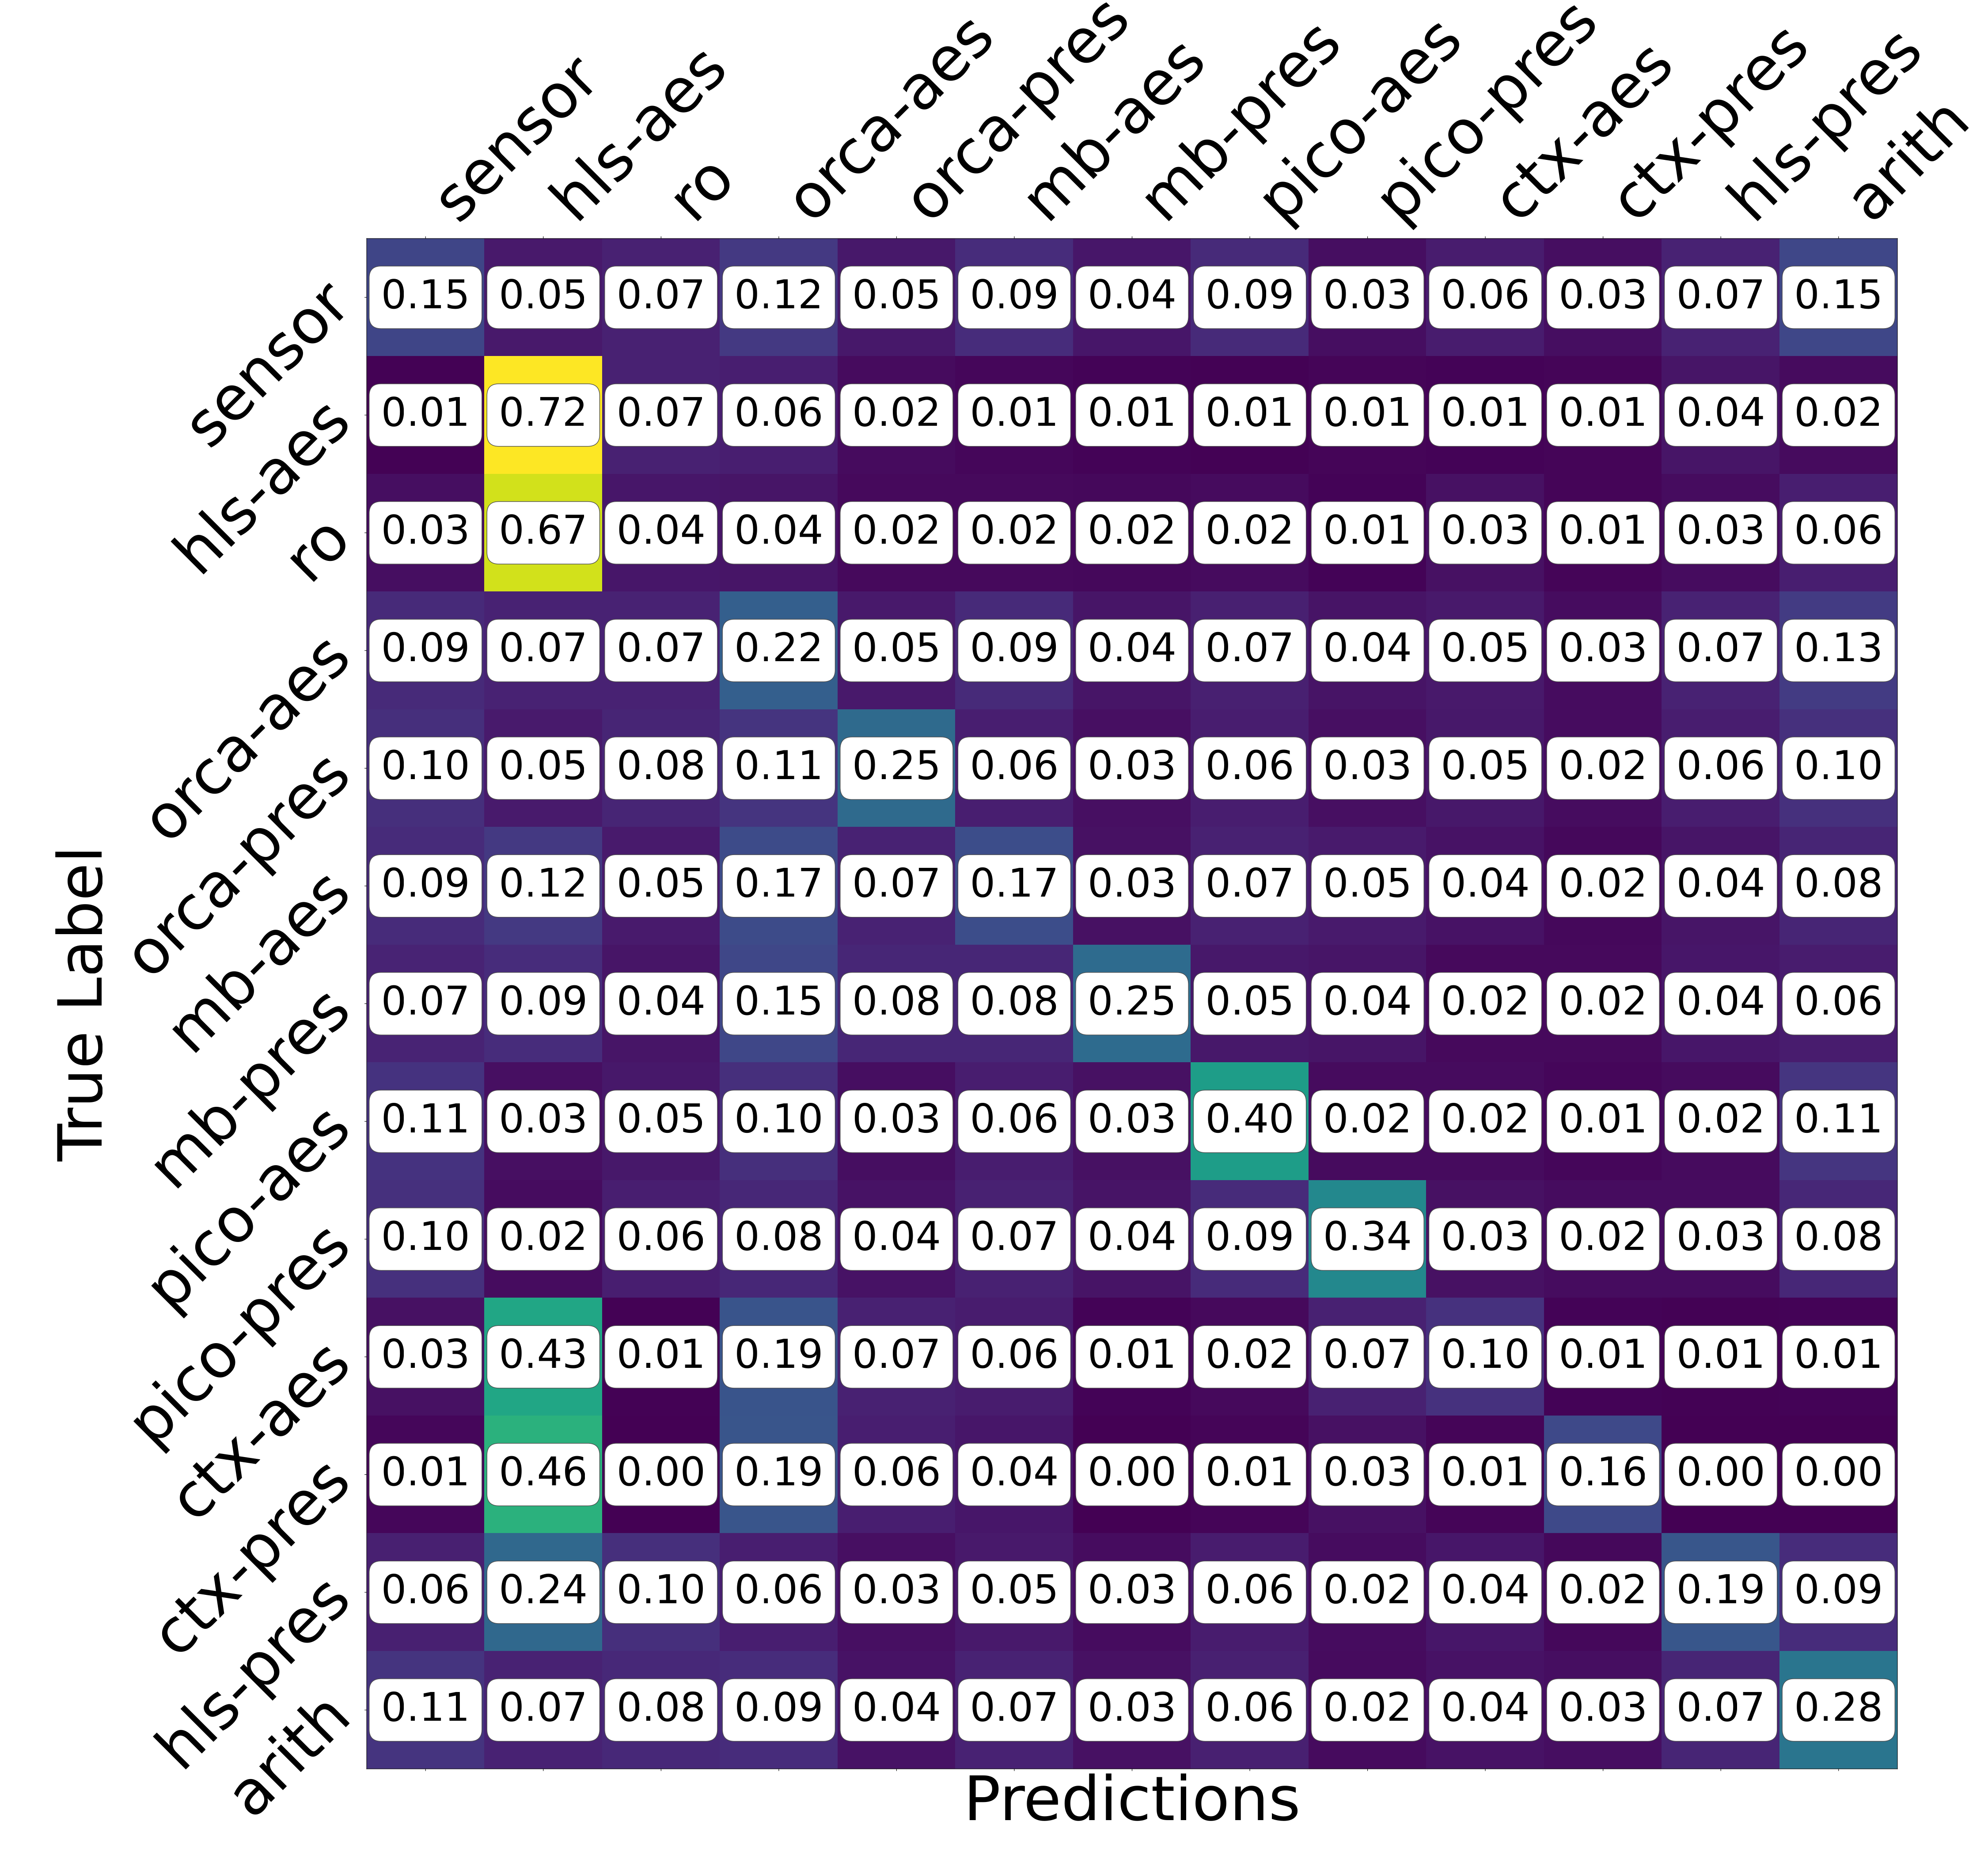
\includegraphics[width=0.45\linewidth]{img/pos-minphi-mintheta-test-board_2e-big-text-confusion-matrix_trimmed.png}\label{classification/rising_min_min}}

% \subfigure[\hspace{10pt}($\downarrow\theta_{max}$, $\phi_{min}$): 51\% accuracy, 1.6$\times$]{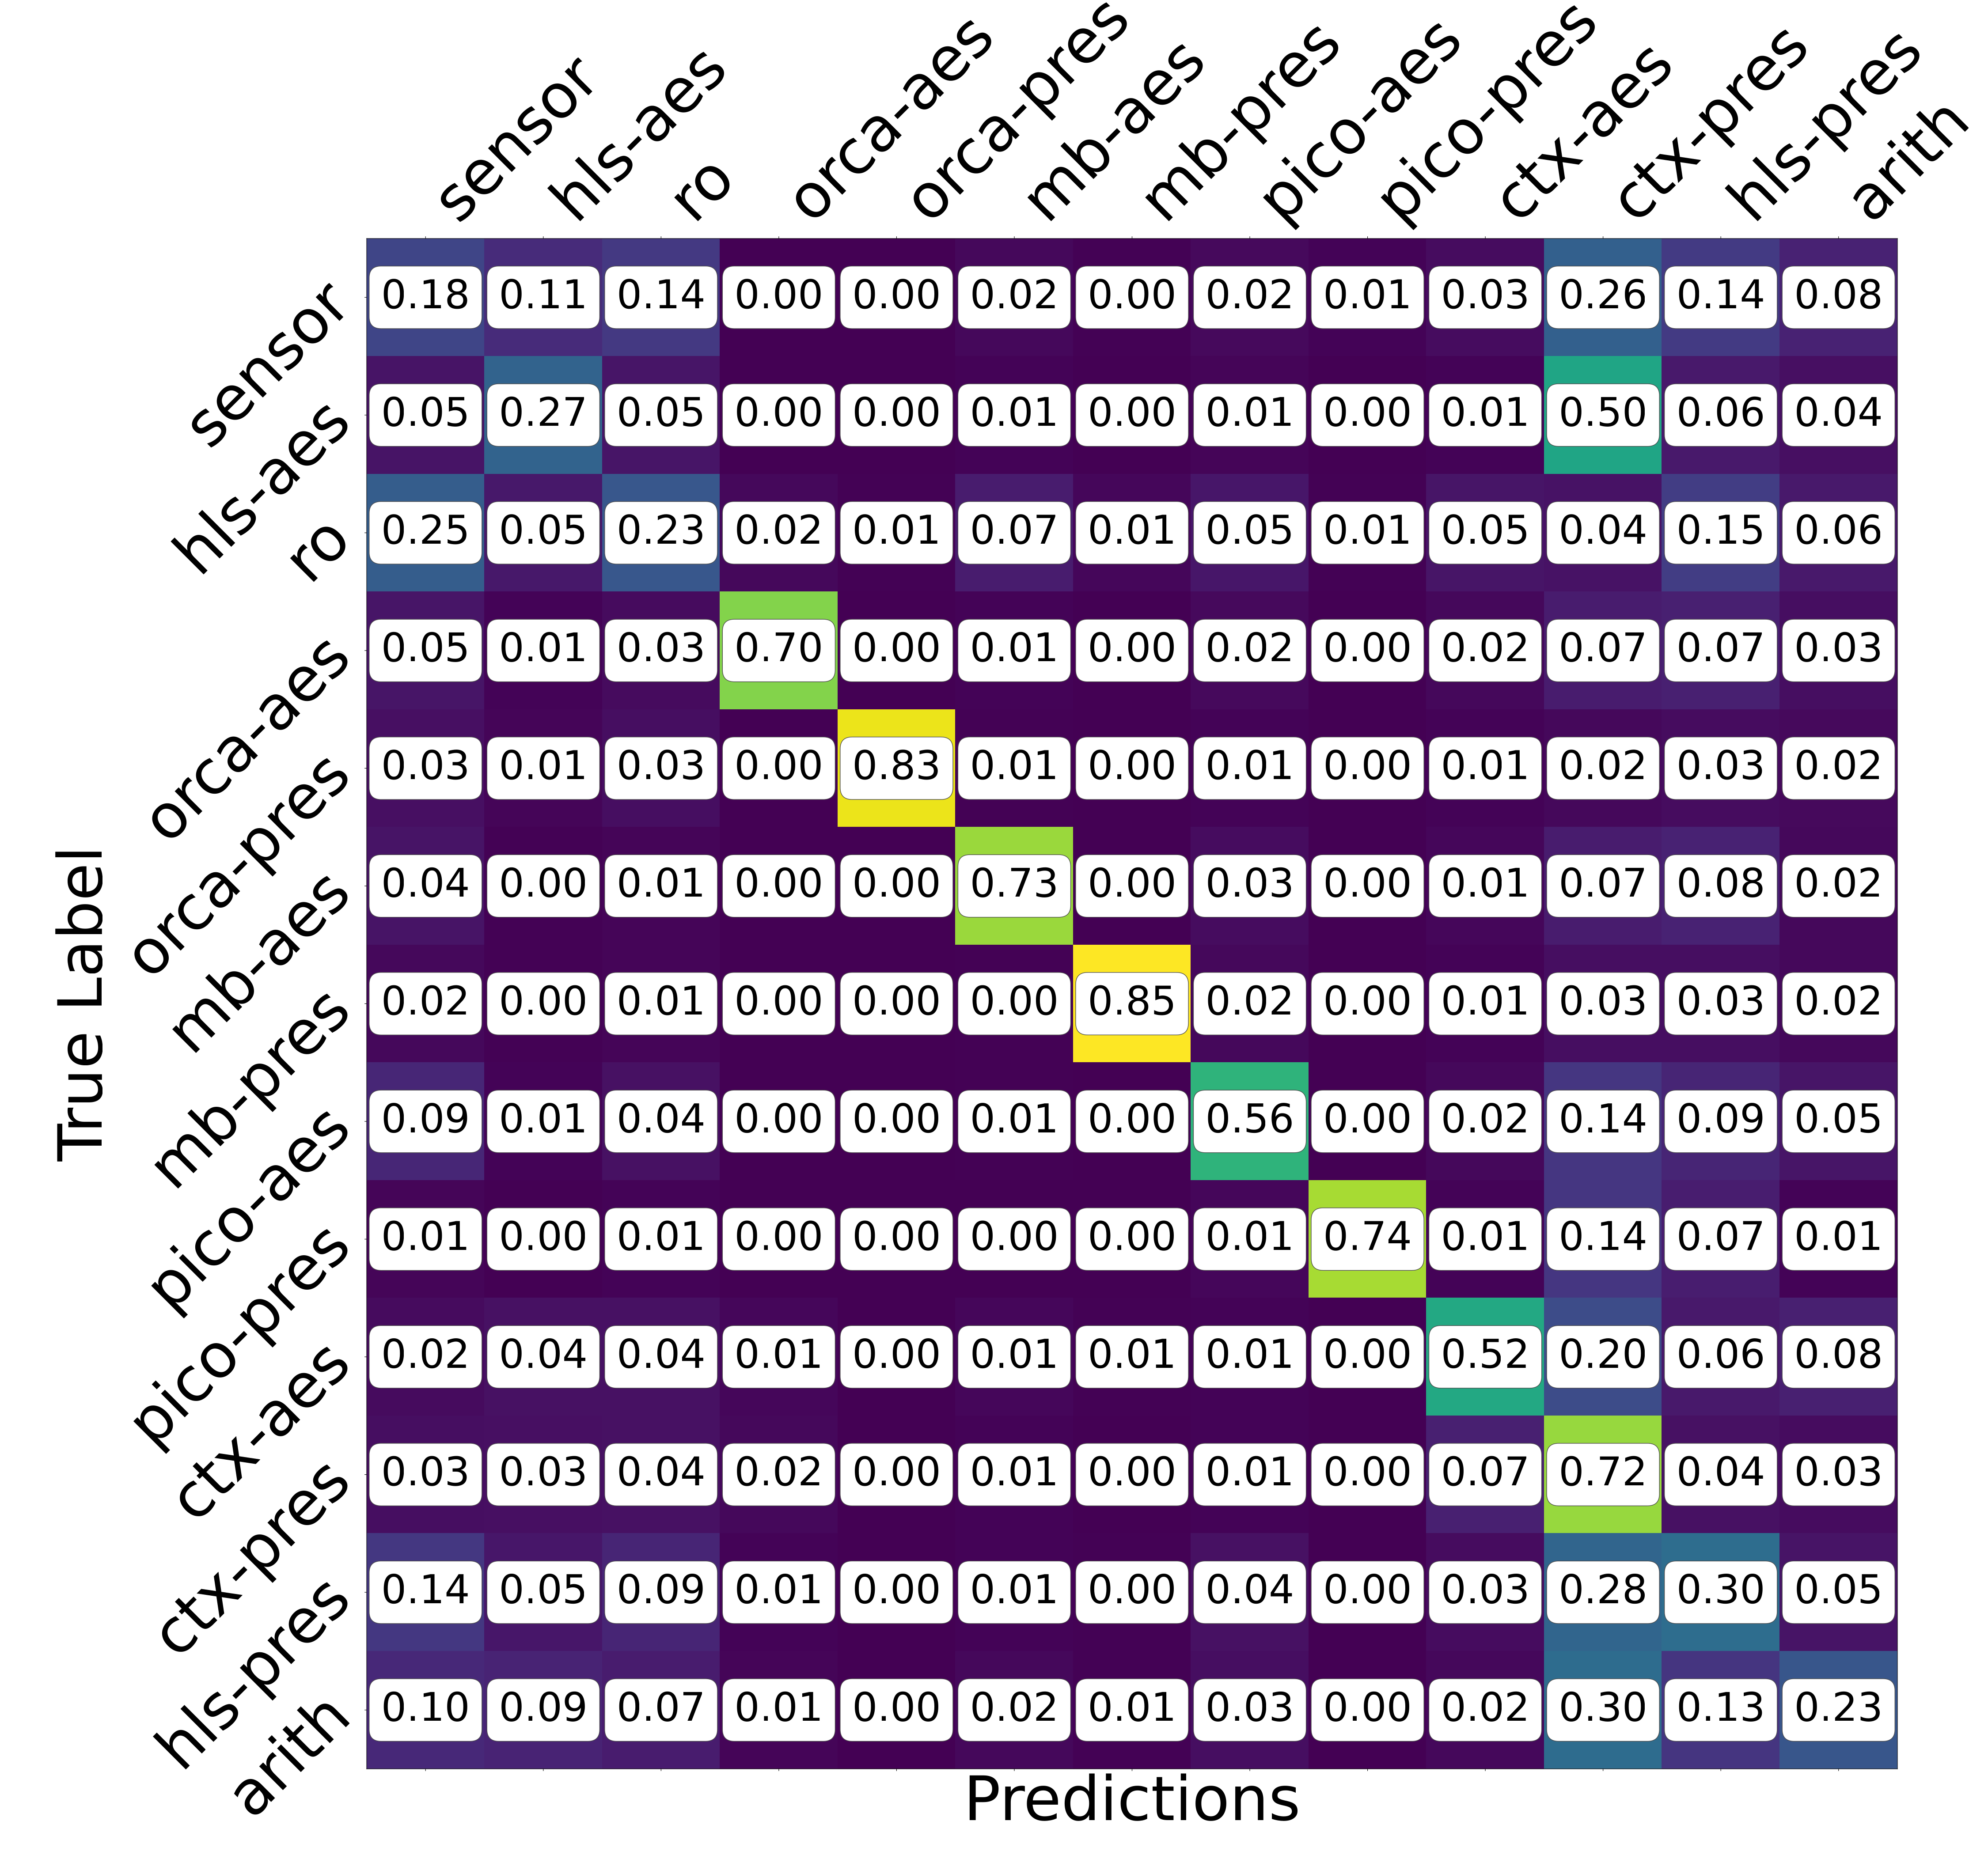
\includegraphics[width=0.45\linewidth]{img/neg-minphi-mintheta-test-board_2e-big-text-confusion-matrix_trimmed.png}\label{classification/falling_min_max}}

% \subfigure[b][\hspace{10pt}($\downarrow\theta_{max}$, $\phi_{back}$): 75\% accuracy, 2.3$\times$]{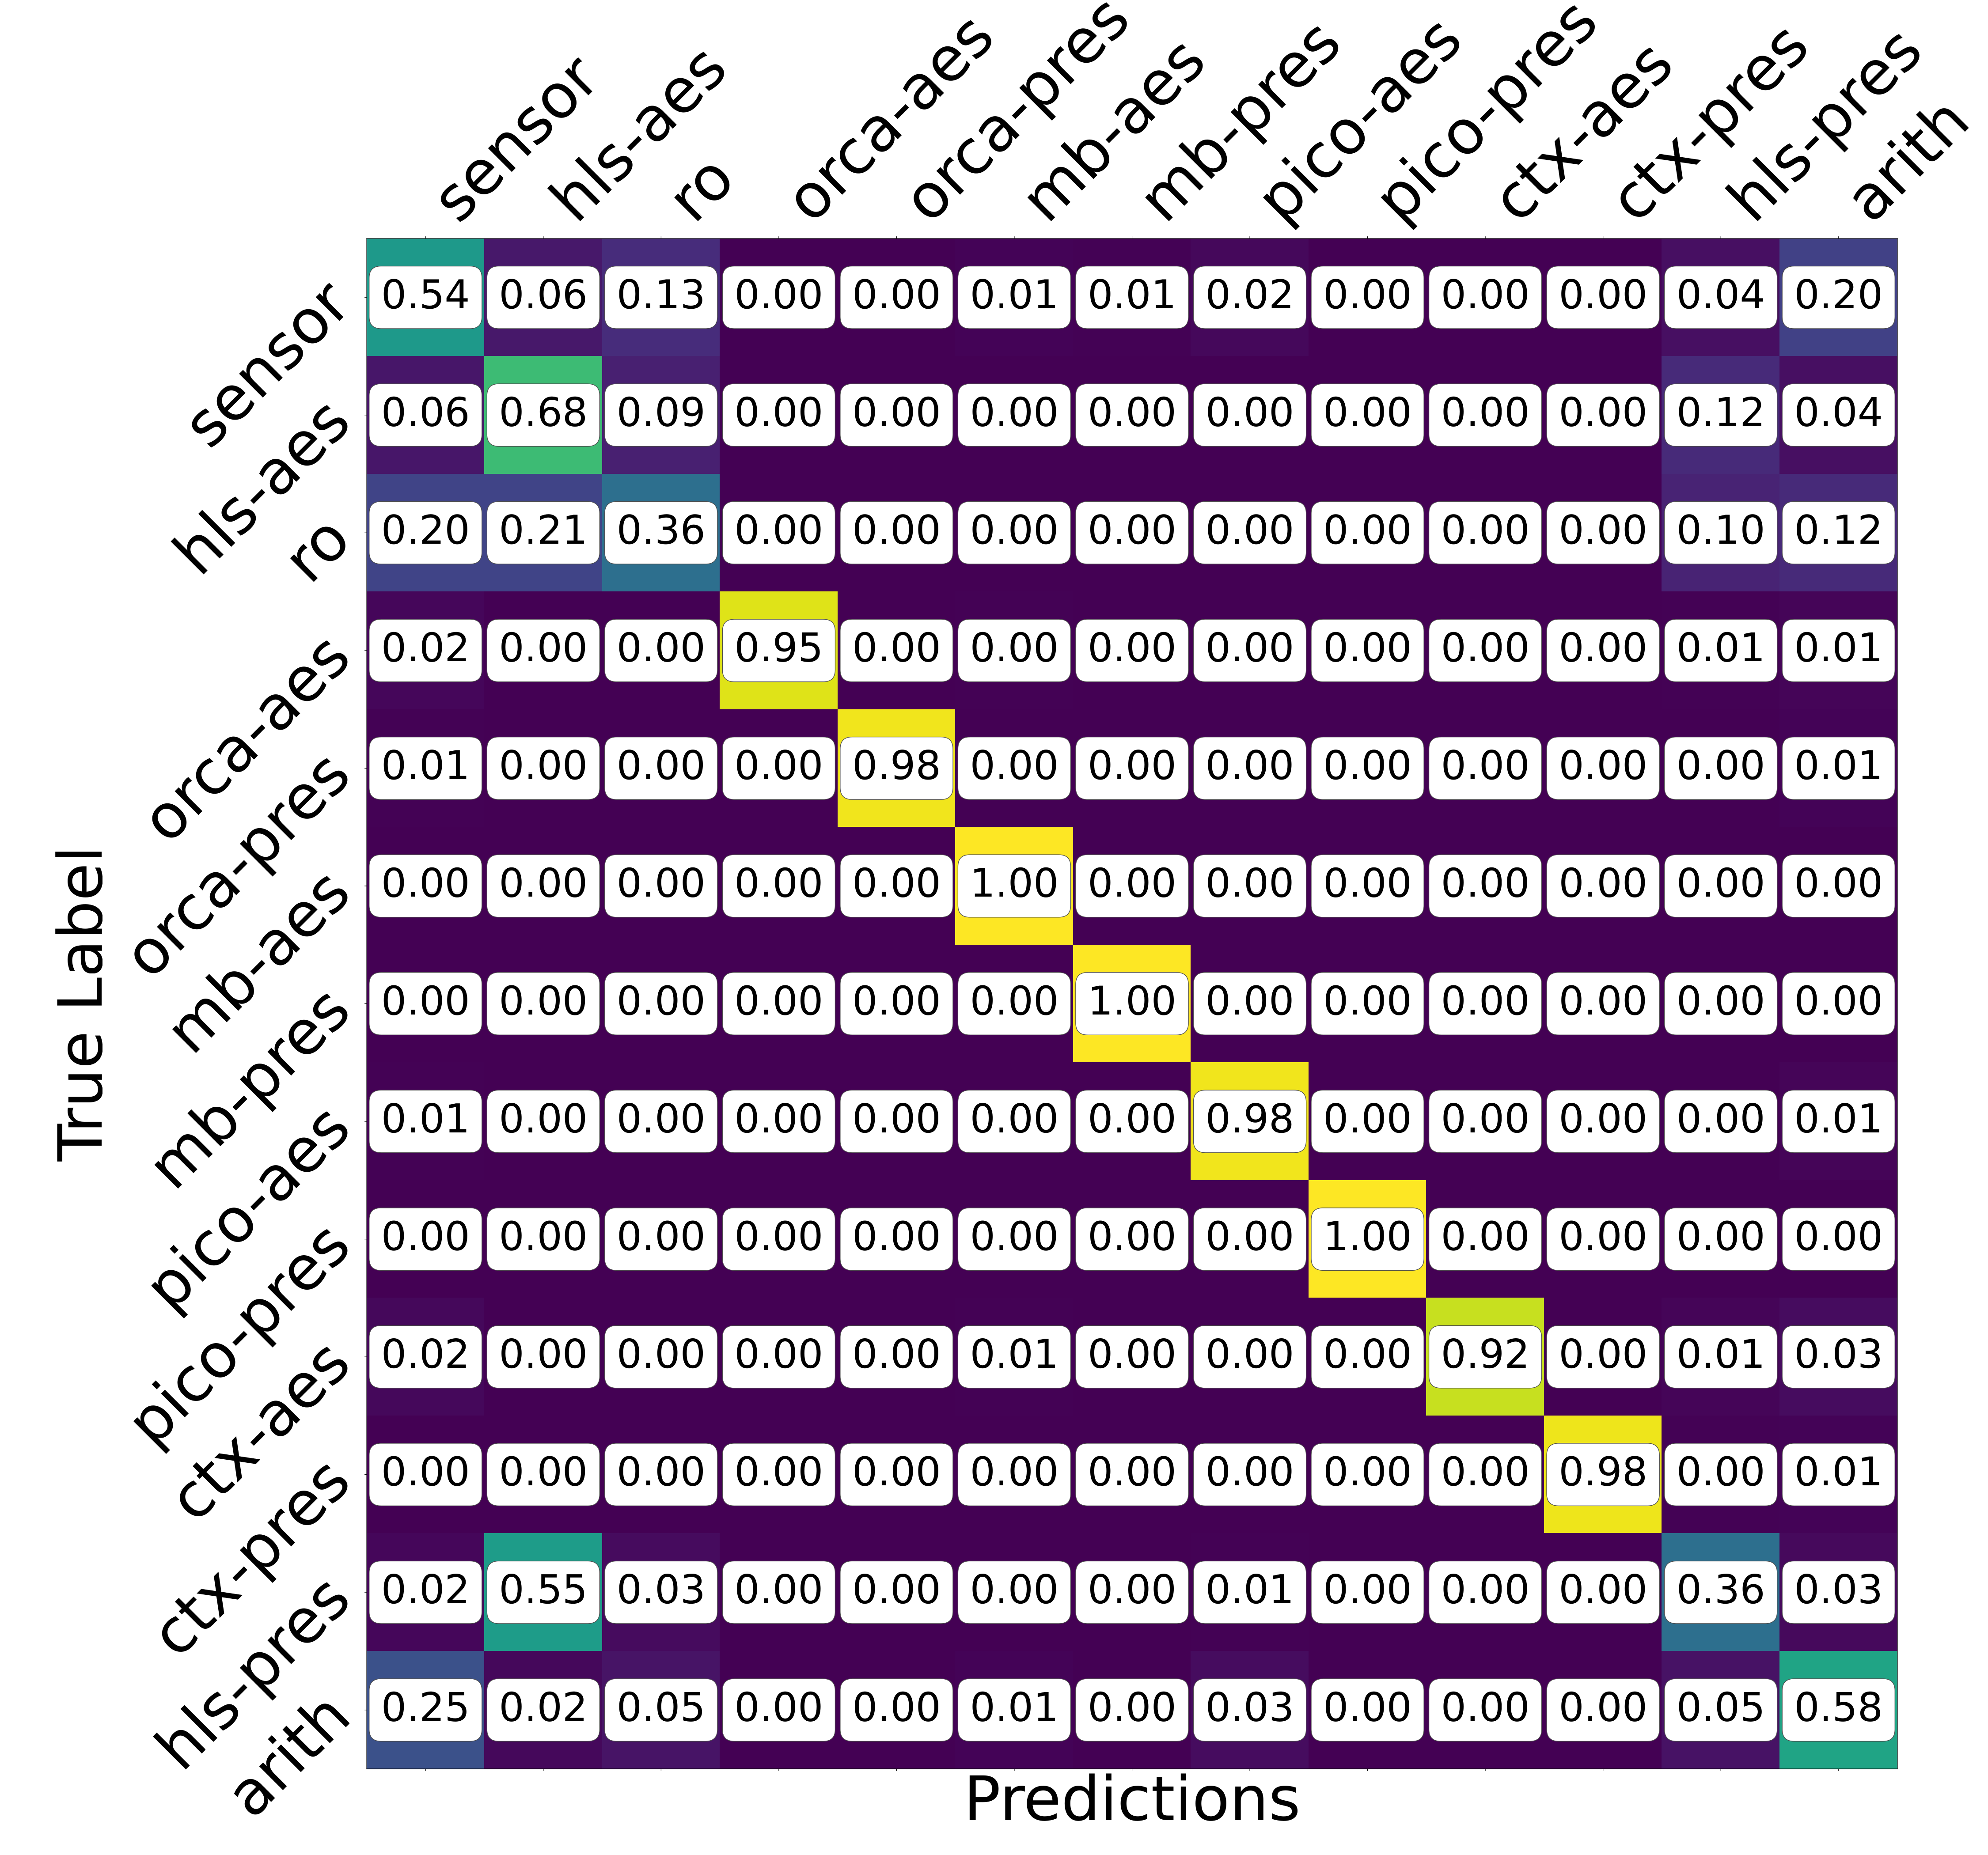
\includegraphics[scale=.043]{img/neg-backsub-maxphi-maxtheta-test-board_fd-big-text-confusion-matrix_trimmed.png}\label{classification/falling_max_max}}

% %\subfigure[($\downarrow\theta_{max}$, $\phi_{back}$)]{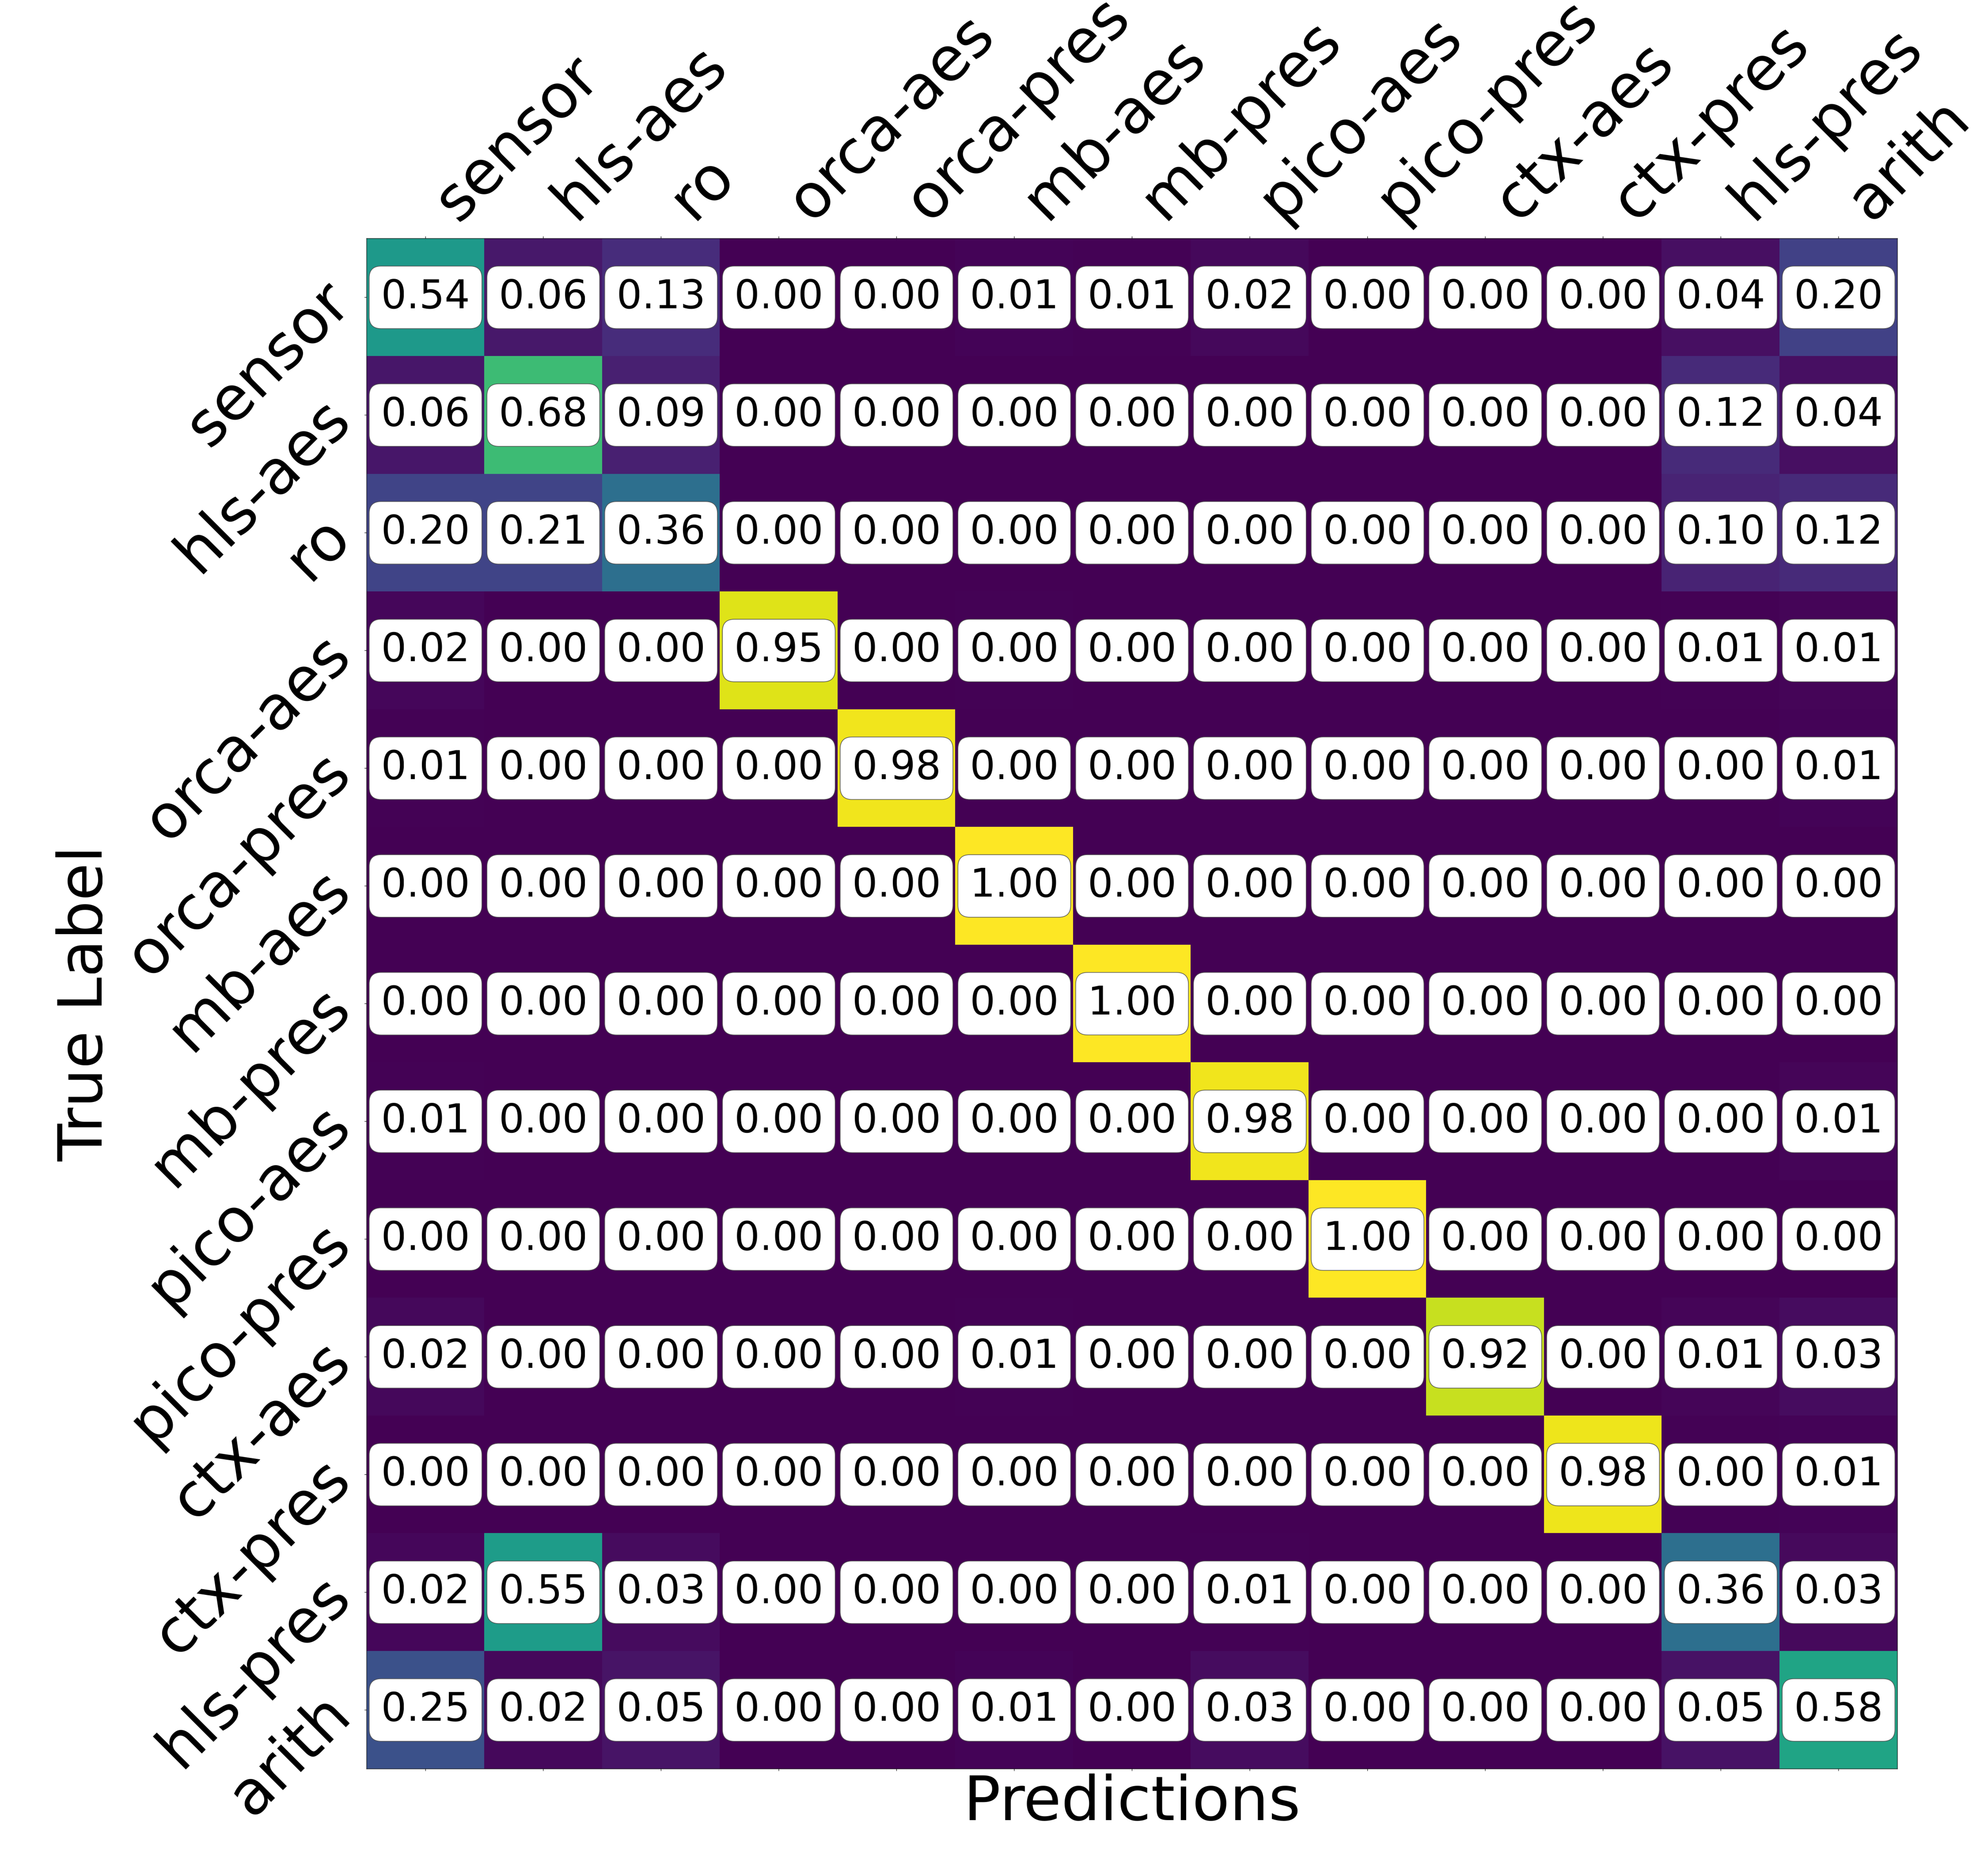
\includegraphics[scale=.09]{img/neg-backsub-maxphi-maxtheta-test-board_fd-big-text-confusion-matrix_trimmed.pdf}\label{classification/falling_max_max}} \\
% \vspace{-15px}
% \caption{Our \name TDC is employed in a 13-way classification task where an attacker extracts the type of co-located computation. The ability to  distinguish co-tenant computations is a measure of side-channel information contained in the sensor's traces.
% %The computations are introduced in Section~\ref{applications}.
% \ref{classification/rising_min_min} represents the worst-case where a TDC cannot reconfigure $\phi$ and $\theta$ and achieves 32\% accuracy. In \ref{classification/falling_min_max} the TDC can tune $\theta$ and improves to 51\% accuracy. In \ref{classification/falling_max_max} both $\theta$ and $\phi$ have been tuned with background subtraction to isolate co-tenant information and achieve 75\% accuracy, a 2.3$\times$ improvement. %\cd{Increase text size if possible. Reduce sig digits if needed}
% }%
% \label{fig:classification-main-figure}%
% \vspace{-10pt}%
% \end{figure*}%

\begin{figure*}[t!]

\begin{minipage}{.5\linewidth}
\centering
\subfloat[\hspace{15pt}($\uparrow\theta_{min}$, $\phi_{min}$): 32\% accuracy, Baseline]{\label{classification/rising_min_min}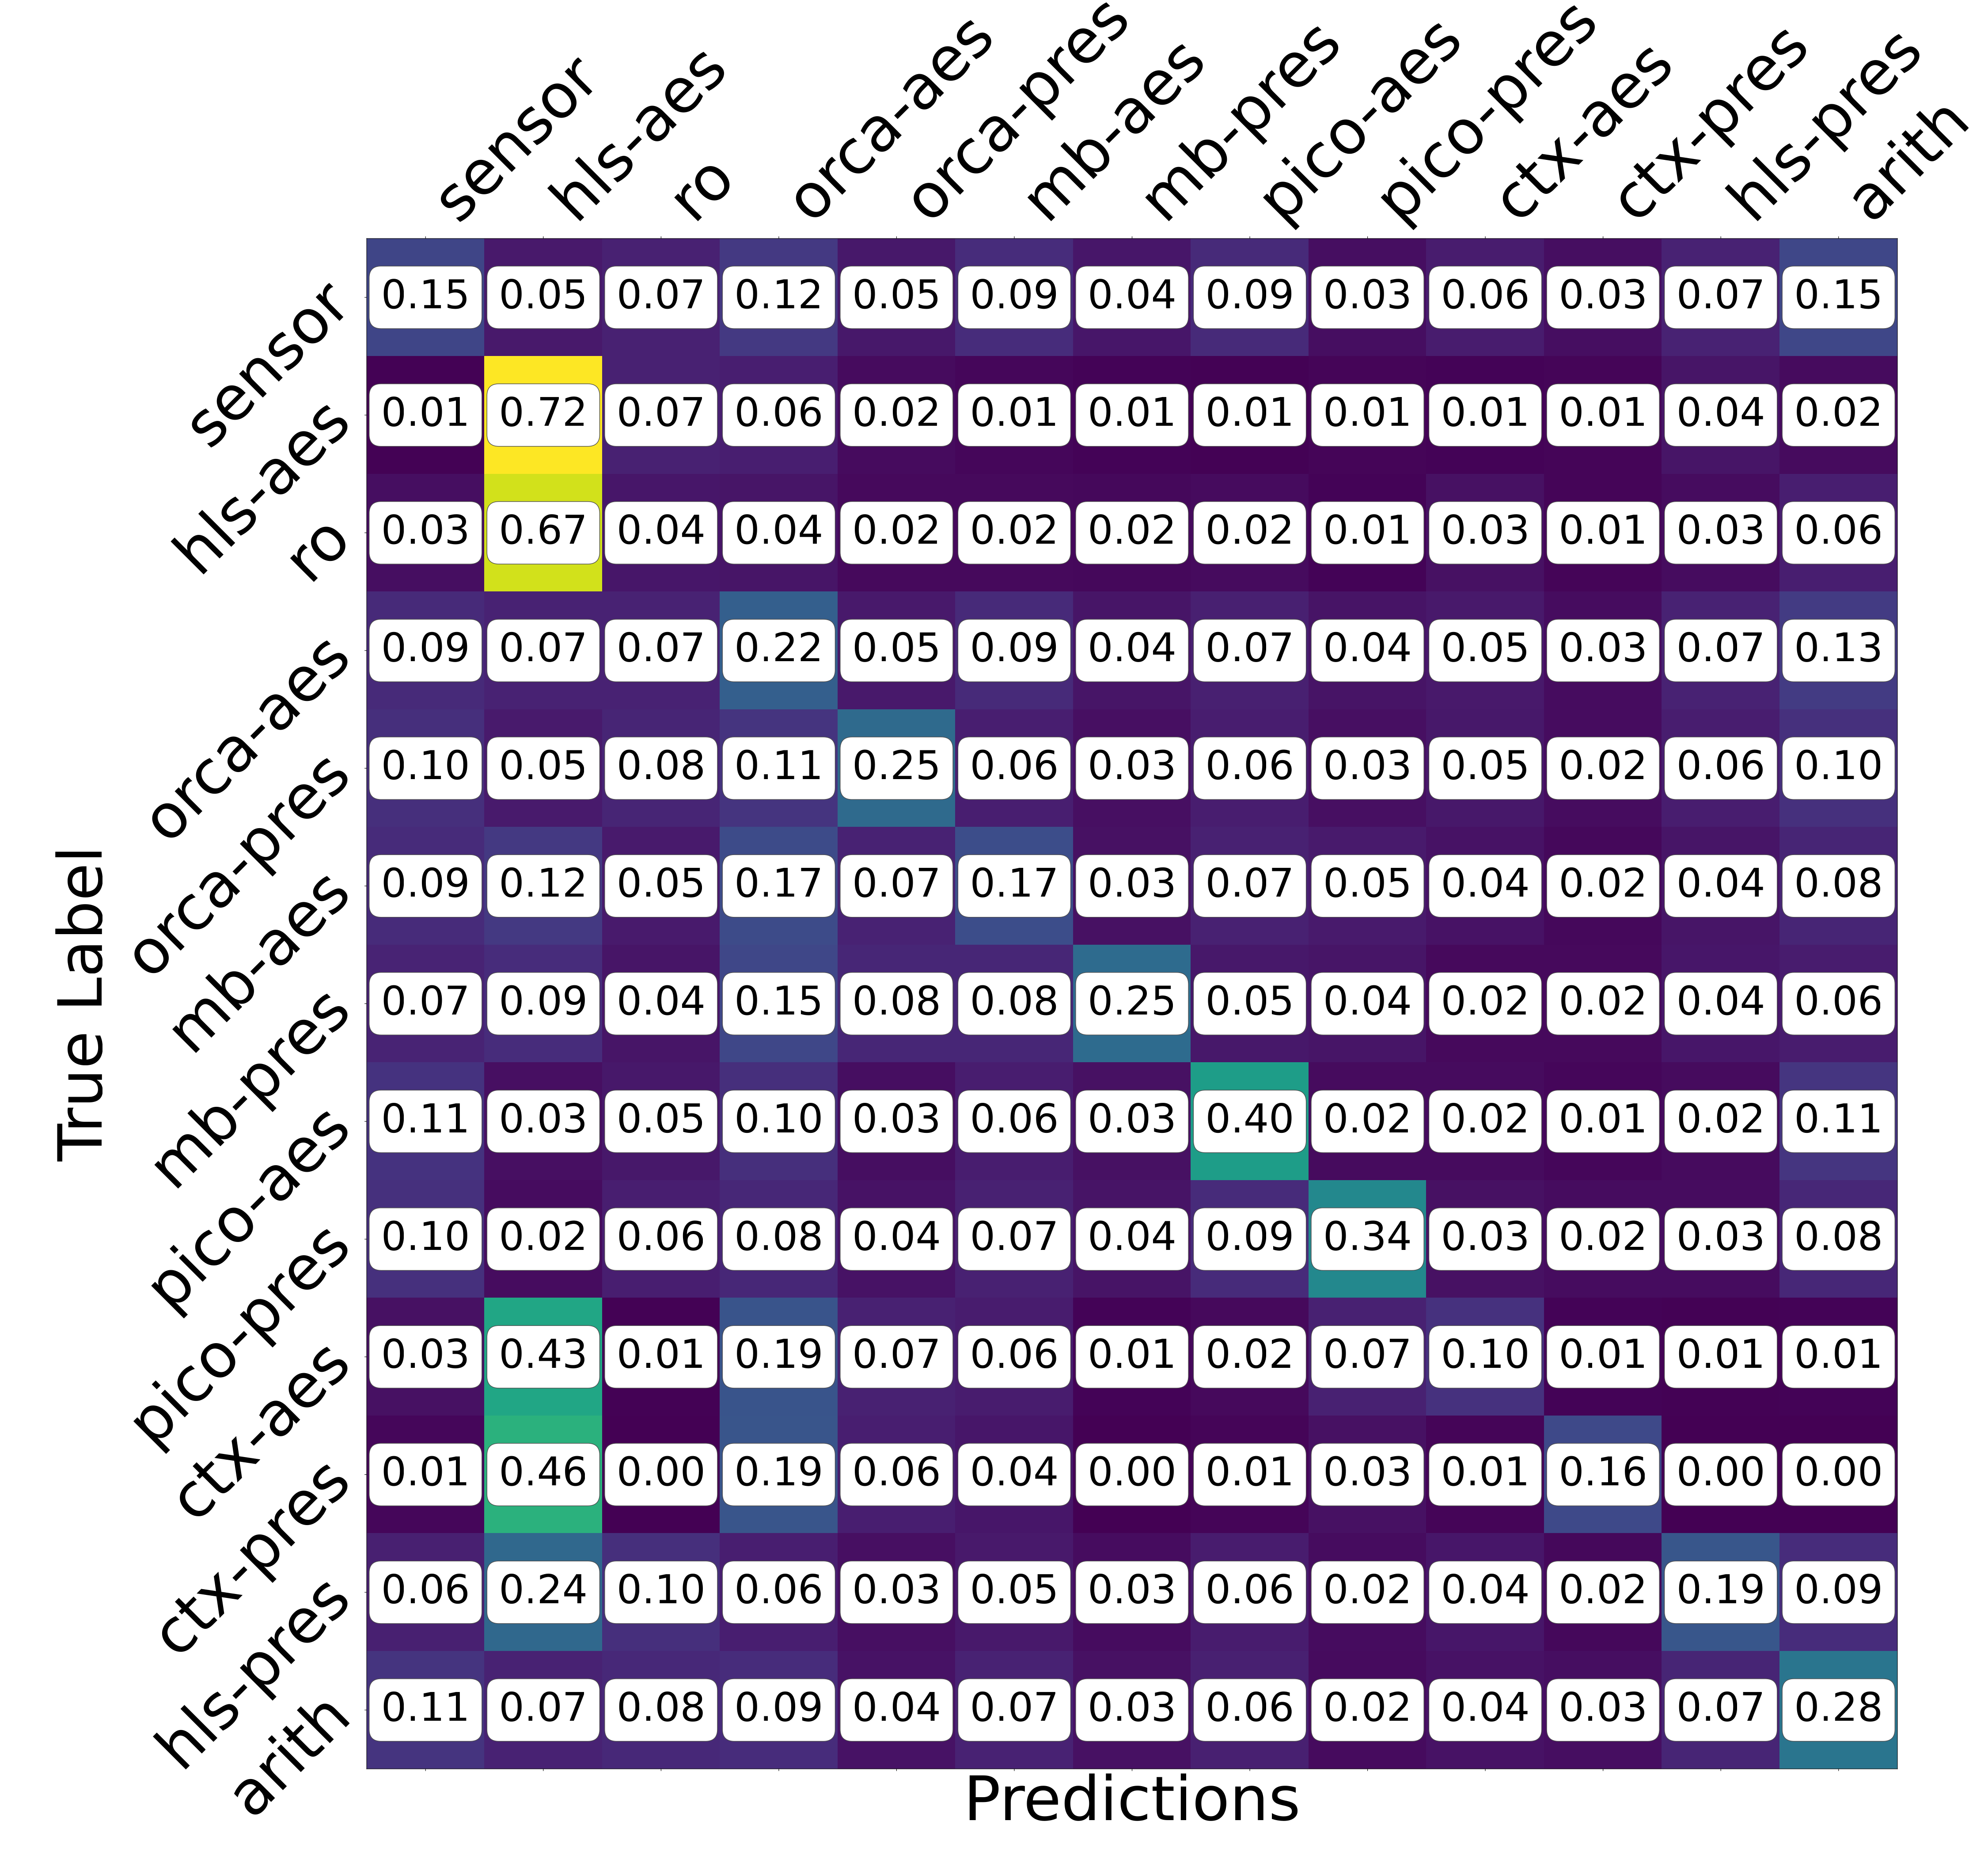
\includegraphics[width=.90\linewidth]{img/pos-minphi-mintheta-test-board_2e-big-text-confusion-matrix_trimmed.png}}
\end{minipage}%
\begin{minipage}{.5\linewidth}
\centering
\subfloat[\hspace{15pt}($\downarrow\theta_{max}$, $\phi_{min}$): 51\% accuracy, 1.6$\times$]{\label{classification/falling_min_max}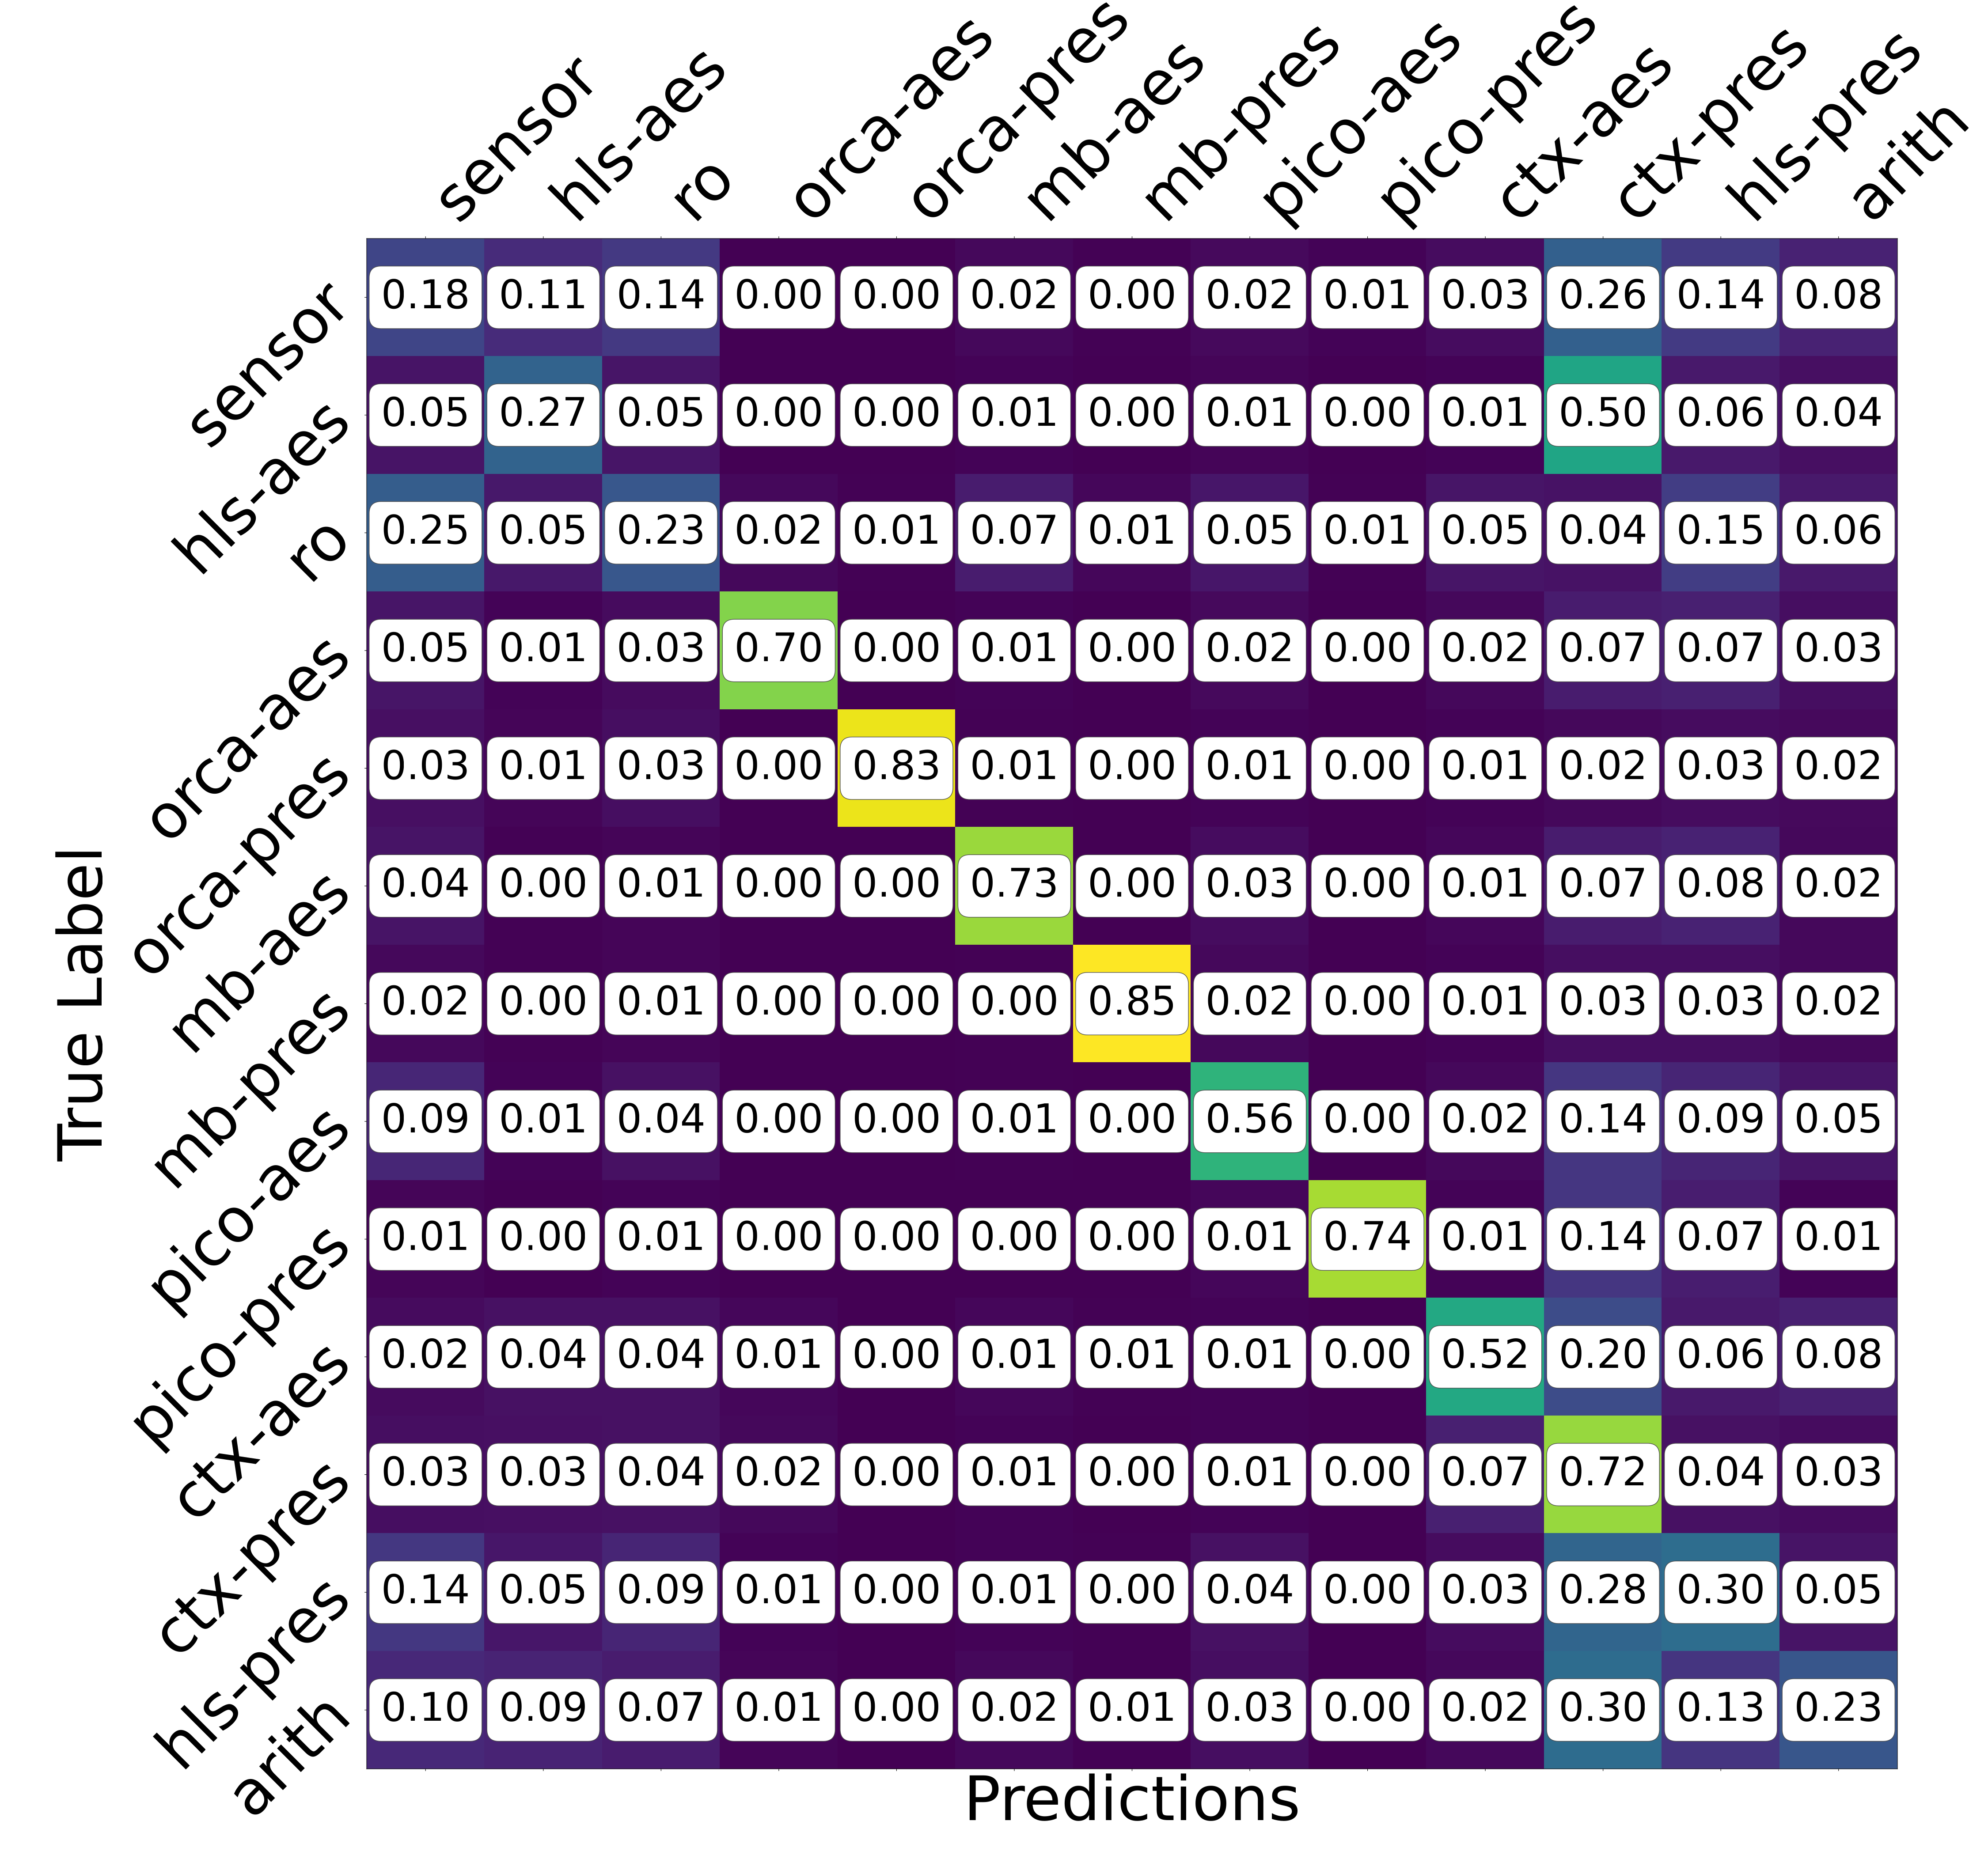
\includegraphics[width=.90\linewidth]{img/neg-minphi-mintheta-test-board_2e-big-text-confusion-matrix_trimmed.png}}
\end{minipage}\par\medskip
\centering
\subfloat[\hspace{15pt}$\downarrow\theta_{max}$, $\phi_{back}$): 75\% accuracy, 2.3$\times$]{\label{classification/falling_max_max}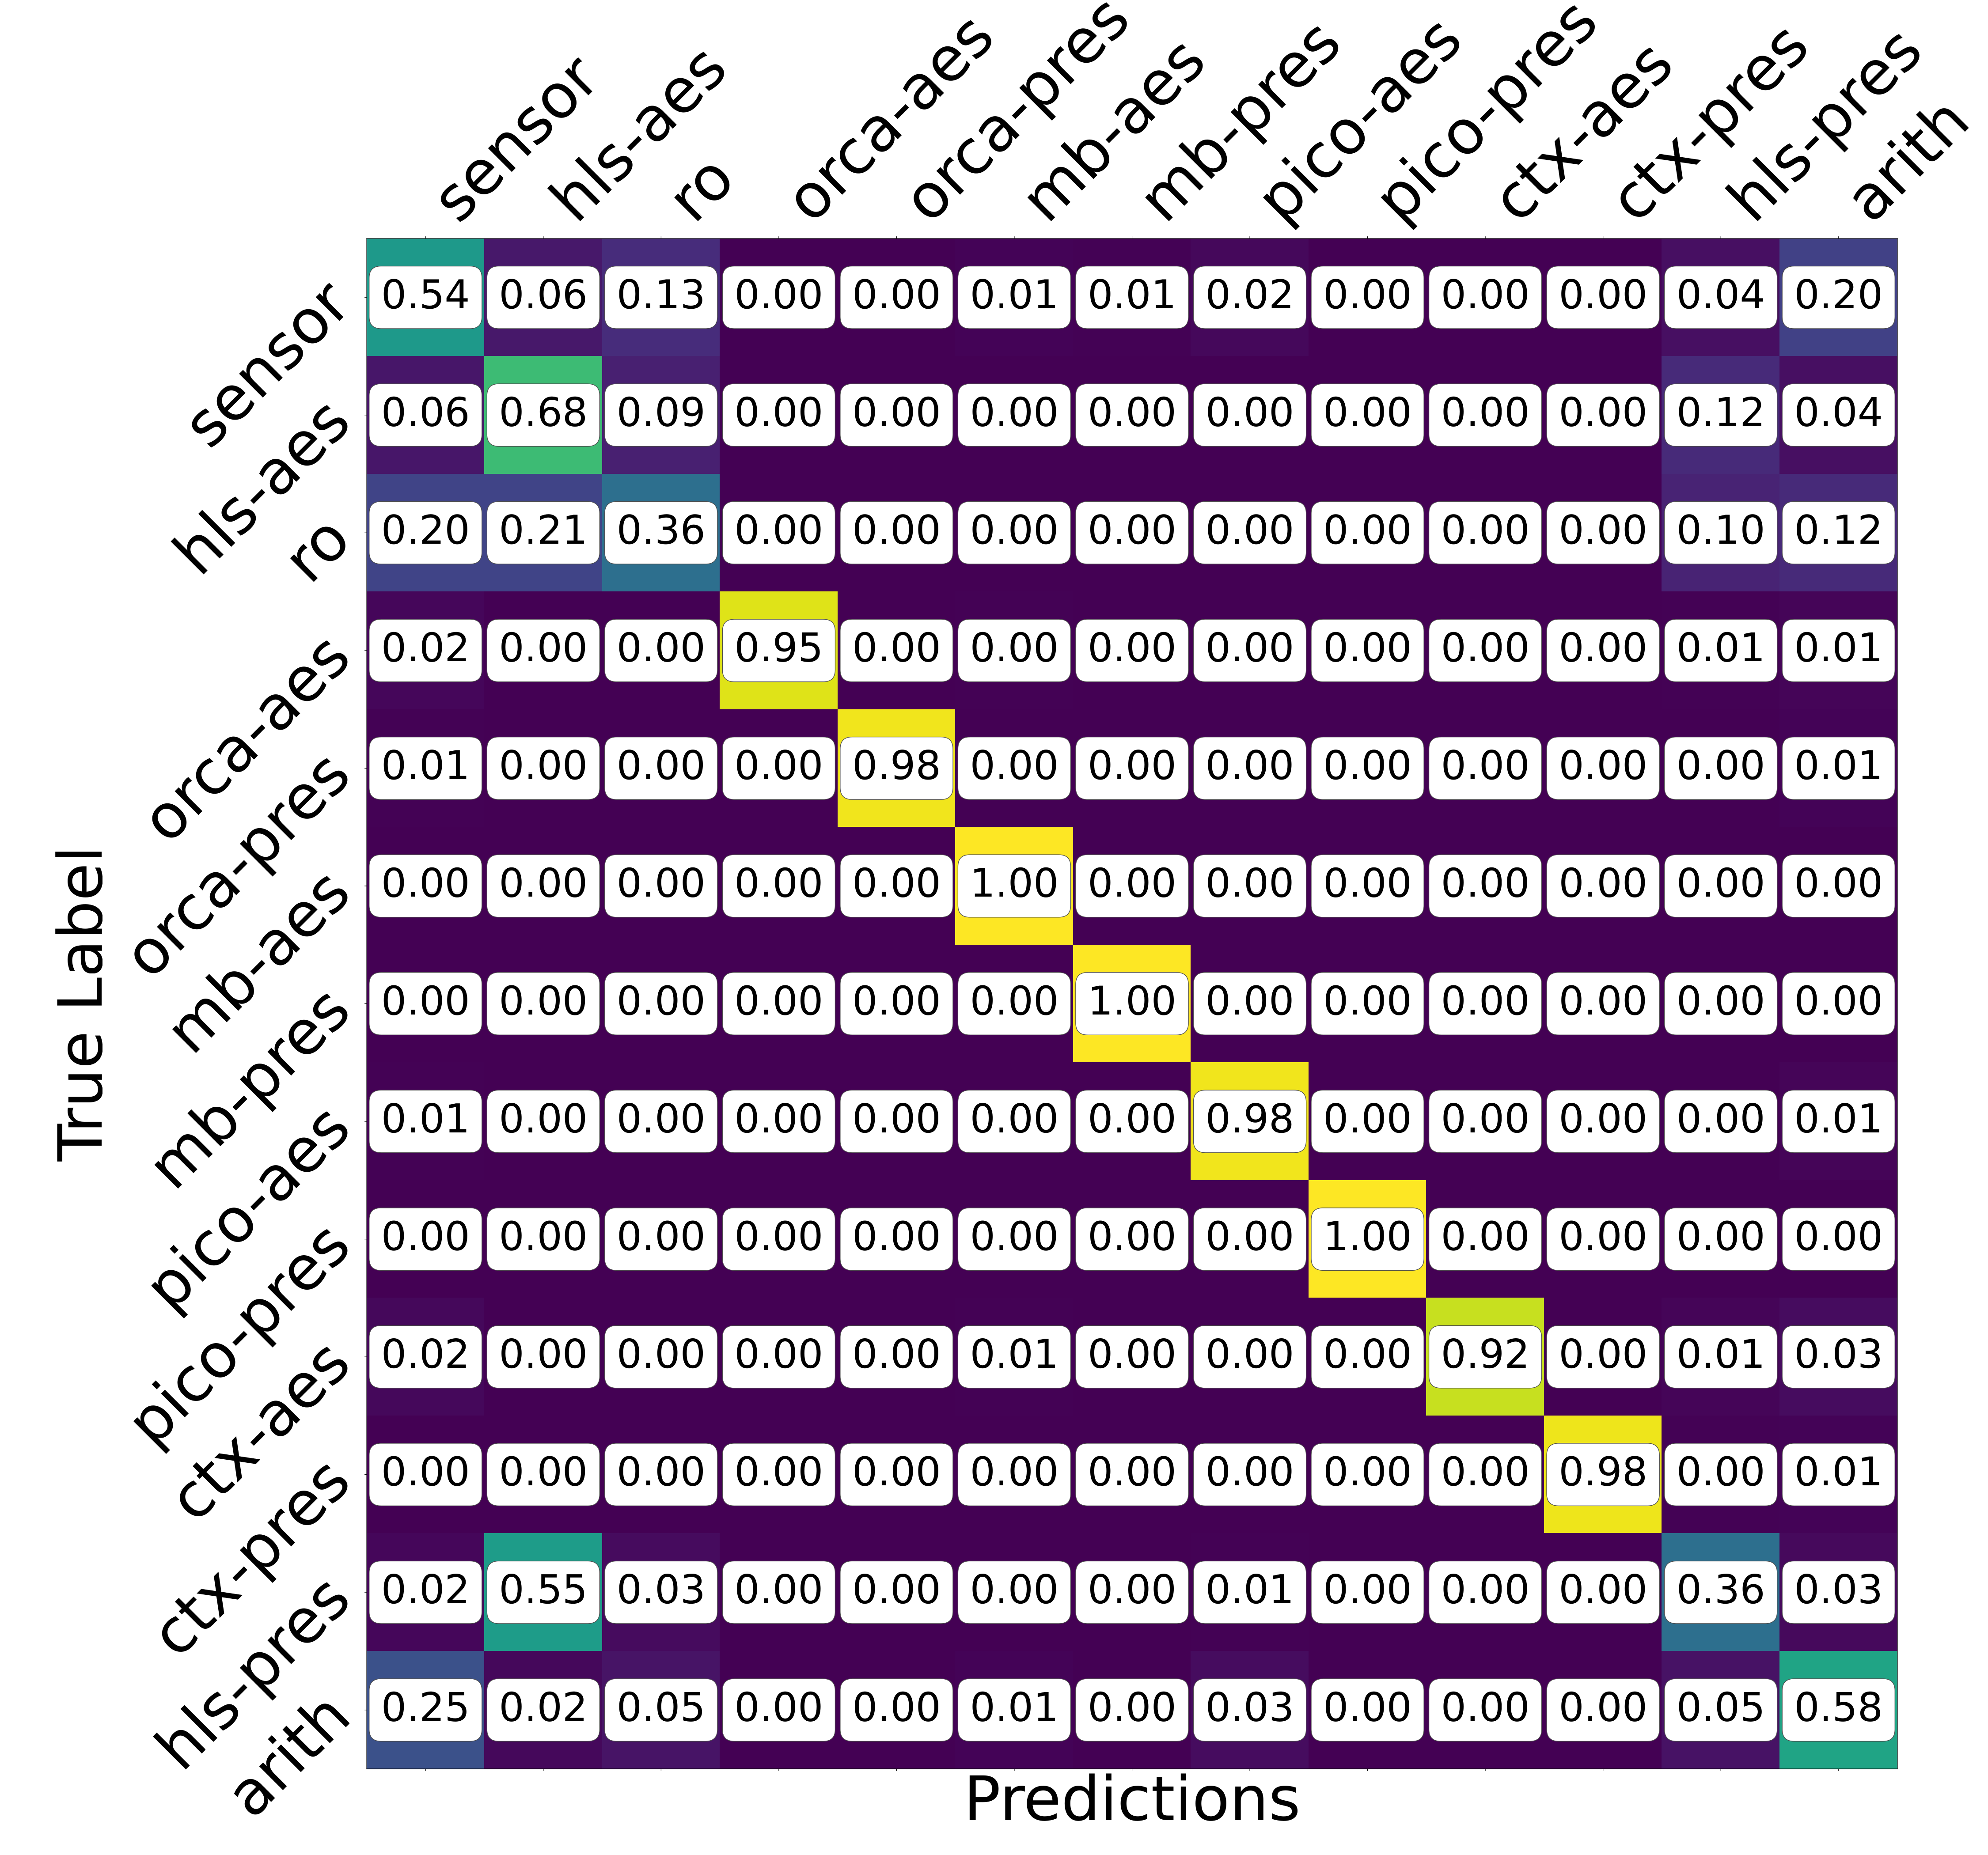
\includegraphics[width=.45\linewidth]{img/neg-backsub-maxphi-maxtheta-test-board_fd-big-text-confusion-matrix_trimmed.png}}

\caption{Our \name TDC is employed in a 13-way classification task where an attacker extracts the type of co-located computation. The ability to  distinguish co-tenant computations is a measure of side-channel information contained in the sensor's traces. The computations are introduced in Section~\ref{applications}. \ref{classification/rising_min_min} represents the worst-case where a TDC cannot reconfigure $\phi$ and $\theta$ and achieves 32\% accuracy. In \ref{classification/falling_min_max} the TDC can tune $\theta$ and improves to 51\% accuracy. In \ref{classification/falling_max_max} both $\theta$ and $\phi$ have been tuned with background subtraction to isolate co-tenant information and achieve 75\% accuracy, a 2.3$\times$ improvement.}
\vspace{-12px}
\label{fig:classification-main-figure}
\end{figure*}

\vspace{-5pt}
\subsection{Effects of Tuning on Classification}
\label{classification}
%As a practical measure of the benefits of tuning, we demonstrate an attack where we accurately classify a co-tenant computation in a multi-tenant system. 
As a precursor to cryptographic key recovery attacks, like a Correlation Power Analysis (CPA), an attacker must be able to determine what and when a cryptographic core is executing. We fill this void by demonstrating an attack where we accurately classify a co-tenant computation in a multi-tenant system. 

% \textcolor{red}{We classify both the encryption algorithm and the architecture the algorithm is implemented on (i.e. HLS, Orca, MicroBlaze, PicoRV, or CortexM3). This is a critical step for an adversary as many key recovery attack parameters may depend on the identified architecture and encryption algorithm. For instance, an adversary could have a priori knowledge of whether or not a switching or hamming distance power model is more effective on a particular architecture. An adversary could also identify cores that are known to leak encryption keys more rapidly, such as Orca, and avoid cores that are more resilient to power side-channel attacks, such as }

%Prior work has demonstrated that co-tenant computations may be identified by collecting training data from \sensor measurements to train classifiers \cite{gobulukoglu2021dac}. However, these attacks have not been deployed in the context of an unknown victim phase and frequency. We will demonstrate that attack efficiency can be improved by tuning the sensor using the methods described in Sections \ref{capture_clock_tuning} and \ref{target_clock_tuning}.

\subsubsection*{\textbf{Setup: }}
As described in Section~\ref{threat_model}, we assume an attacker uploads a \sensor to a remote multi-tenant FPGA environment to extract the architecture and algorithm of co-tenant computation through the comparison of captured power traces to a known body of labeled training data. 
This training data can be generated in two possible ways. First, a malicious actor, utilizing two separate user accounts, can instantiate a \sensor with one user and attempt to co-locate with the second user, which instantiates a known design. 
This would allow an attacker to build a data set on the same architecture where the attack will be performed. The second option is to create a data set using local boards of the same type as the cloud environment.
Because this choice depends on the implementation details of the multi-tenant model, we will not consider this in our analysis. 
Such an attack serves as a violation of the application anonymity guaranteed by such a multi-tenant system.
The attack is performed on each of the 13 applications on 5 PYNQ-Z2 platforms.

%As a practical measure of the side-channel capacity gained with our sensor and its proper calibration, we consider the ability of an attacker to classify the type of co-tenant computation accurately. As described in our threat model (Section~\ref{threat_model}), an attacker uploads a \sensor to a remote multi-tenant FPGA environment to extract the type of co-tenant computation. Such an attack violates application anonymity and acts as a precursor to existing multi-tenant side-channel exploits, e.g., a DPA attack relies on the knowledge of the existence of a cryptographic core. 


%\subsubsection{Experimental Setup}
%\vspace{5pt}
\paragraph{$\theta$ Tuning: }
In the following experiment we consider four configurations of $\theta$: $\uparrow\theta_{max}$, $\uparrow\theta_{min}$, $\downarrow\theta_{max}$, and $\downarrow\theta_{min}$.
We sweep through the 64-bit delay line and record a trace's average and standard deviation at each point.
The position where standard deviation has been maximized for a particular rising/falling transition polarity we call $\uparrow\theta_{max}$ / $\downarrow\theta_{max}$, and the point where standard deviation has been minimized for a particular rising/falling transition polarity we call $\uparrow\theta_{min}$ / $\downarrow\theta_{min}$. 

%The point at which standard deviation is maximized (minimized) in the rising and falling transition we label $\uparrow\theta_{max}$ ($\uparrow\theta_{min}$) and $\downarrow\theta_{max}$ ($\downarrow\theta_{min}$) respectively. 
%\vspace{5pt}
\paragraph{$\phi$ Tuning: }
The sensor's $\phi$ will be configured three ways: first at a state of absolute maximum standard deviation ($\phi_{max}$), at its absolute minimum standard deviation ($\phi_{min}$), and finally the maximum standard deviation under the background subtraction ($\phi_{back}$) process of Section~\ref{target_clock_tuning}.
Just as in Section~\ref{target_clock_tuning}, $\phi$ is shifted in 14.88~ps increments 2688 times at each point, capturing a trace of 128 samples---once to capture background noise ($\sigma_{back}$), and again once the target application has been enabled ($\sigma_{active}$).
In the tuning process, $\phi_{max}$ ($\phi_{min}$) is the maximum (minimum) standard deviation of the $\sigma_{active}$ sweep for a given transition type. The position of maximum standard deviation after background tuning ($\phi_{back}$) is the maximum standard deviation of $\sigma_{active}-\sigma_{back}$.

% \vspace{5pt}
\paragraph{Data Collection: }
The target design and sensor are loaded onto the device. Then, $\theta$ is positioned at one of $\uparrow\theta_{max}$, $\downarrow\theta_{max}$, $\uparrow\theta_{min}$, or $\downarrow\theta_{min}$. Finally, $\phi$ is configured to one of $\phi_{max}$, $\phi_{min}$, or $\phi_{back}$.

We examine the following tuning combinations of ($\theta$, $\phi$): ($\uparrow\theta_{min}$, $\phi_{min}$) emulates the worst-case of a non-tunable TDC. ($\downarrow\theta_{max}$, $\phi_{min}$) introduces $\theta$ tuning to demonstrate how the mitigation of carry-chain non-linearity improves the sensor’s ability to resolve co-tenant information. ($\downarrow\theta_{max}$, $\phi_{max}$) demonstrates the significance of $\phi$ tuning on classification accuracy. ($\downarrow\theta_{max}$, $\phi_{back}$) demonstrates how background subtraction improves our ability to optimize the co-tenant side channel. ($\uparrow\theta_{max}$, $\phi_{back}$) is used to determine which transition polarity captures the most information, as it can be directly compared against ($\downarrow\theta_{max}$, $\phi_{back}$).
%($\downarrow\theta_{max}$, $\phi_{max}$), ($\downarrow\theta_{max}$, $\phi_{back}$), ($\downarrow\theta_{max}$, $\phi_{min}$), ($\uparrow\theta_{max}$, $\phi_{max}$), and ($\uparrow\theta_{min}$, $\phi_{min}$).

%\begin{enumerate}
%    \item \textbf{($\uparrow\theta_{min}$, $\phi_{min}$):} This emulates the worst-case of a non-tunable TDC.% In a non-tunable TDC attack scenario $\phi$ is random at initialization. Because $\phi$ may be positioned anywhere on the spectrum 0 to $2\pi$, we pick the case when the standard deviation is minimized for the rising transition. Depending on the static load on the PDN, a poor $\theta$ may cause the transition to fall on a plateau. This serves as a baseline to show how information recovery can be improved with proper tuning.

%    \item \textbf{($\downarrow\theta_{max}$, $\phi_{min}$):} This introduces $\theta$ tuning to demonstrate how to begin able to mitigate carry-chain non-linearity improves the ability of the sensor to resolve co-tenant information.
    
 %   \item \textbf{($\downarrow\theta_{max}$, $\phi_{max}$):} This dataset demonstrates significance of $\phi$ tuning on classification accuracy.

%    \item \textbf{($\downarrow\theta_{max}$, $\phi_{back}$):} This dataset demonstrates how background subtraction improves our ability to optimize the co-tenant side channel. 
    
%    \item \textbf{($\uparrow\theta_{max}$, $\phi_{back}$):} To determine which transition polarity captures the most information, we generate a data set to compare against ($\downarrow\theta_{max}$, $\phi_{back}$).
%\end{enumerate}
After the sensor is configured, the target computation is launched, and a trace of $2^{16}$ samples are gathered. This process is repeated 100 times on each application for a total of 1300 traces per tuning combination per board. \footnote{All of the data sets for each of the 13 applications, for each of the five boards, for each of the five tuning methods, along with the entire classification pipeline and network details are available at: https://github.com/KastnerRG/multitenant-classification} 

%\vspace{-50px}

\begin{comment}
\begin{table*}[ht!]
\centering
\caption{All prior work implements a subset of our sensor's capabilities, which can be related to the ordered tuple in ``$\star$ Tuning''. Each tuning can then be related to a classification accuracy (\%)/loss as well as the GSR @ 50K traces, PSR (Min, Avg, Max) @ 50K, and PGE (Min, Avg, Max) @ 50K. No prior experiments have measured how well information learned on one board can generalize to other boards of the same type (called cross-board or XB) as we do---a crucial consideration for cloud attacks. ($\star$ = This Work)}\label{table:relatedwork}\label{table:classification}\label{table:cpastats}
\begin{tabular}{llllllll}
Literature & XB & $\star$ Tuning & \% & Loss & GSR & PSR & PGE \\
\hline
\cite{gobulukoglu2021dac,schellenberg2018inside,schellenberg2018remote, gnad2017voltage} & \xmark & ($\uparrow\theta_{min}$, $\phi_{min}$) & 32.146\% &  2.159 & 0\% & (5\%, 23\%, 45\%) & (54.8, 87.2 126.2) \\
\cite{favi200917ps,krautter2020cpamap,daigneault2011high,zick2013sensing,glamovcanin2020cloud} & \xmark & ($\downarrow\theta_{max}$, $\phi_{min}$) & 51.160\%  & 1.644 & NA & NA & NA \\
$\star$ & \cmark & ($\downarrow\theta_{max}$, $\phi_{max}$)  & 75.788\%  & 0.834 & NA & NA & NA\\
$\star$ & \cmark & ($\downarrow\theta_{max}$, $\phi_{back}$) & 75.552\% & 0.733  & NA & NA & NA  \\
$\star$ & \cmark & ($\uparrow\theta_{max}$, $\phi_{back}$)   & 80.943\% & 0.668  & 5\% & (15\%, 48\%, 90\%) & (0.8, 46.9, 95.4)  
\end{tabular}
\end{table*}
\end{comment}

\paragraph{Post-processing:}
For a group of 1300 traces from a single tuning configuration ($\theta$, $\phi$) on a single board, we randomly segment each trace into ten sub-traces of $2^{13}$ samples. Each sub-trace is de-trended to remove the DC offset. The Fourier transform of the processed trace is then computed. From an original set of 1300 traces, we are left with 1000 rising transition Fourier transforms and 1000 falling transition Fourier transforms for each application, amounting to 26000 Fourier transforms per board per configuration.

\paragraph{Network Architecture:}
We train a simple neural network of only one fully connected layer, a fast and simplistic starting point. We evaluate the classification accuracy (how accurately our network can classify among the 13 classes of computation) and cross-entropy loss (how well our network generalizes to unseen data) on all configurations of training on four boards and testing on a 5th. 

%Each scenario has a different set of 4 training boards and a 5th testing board. The classification accuracy is a measure of how accurately our network can classify among the 13 classes of computation. Cross-entropy loss indicates how well our network generalizes to unseen data, as it measures how far away the model's predictions are from the true labels. A perfect model would have a loss of 0.

\subsubsection*{\textbf{Classification Results:}}
The results of our experiments are shown in Table~\ref{table:classification}, and select confusion matrices from our 13-way experiment are shown in Figure~\ref{fig:classification-main-figure}. The results are summarized below: 


%\begin{table}[h]
%\centering
%\caption{Average accuracy and loss across configurations.}\label{table:classification}

%\begin{tabular}{lcc}
%Tuning                                 & Accuracy (\%) & Loss  \\
%\hline
%($\uparrow\theta_{min}$, $\phi_{min}$) & 32.146 & 2.159 \\
%($\downarrow\theta_{max}$, $\phi_{min}$) & 51.160 & 1.644 \\
%($\downarrow\theta_{max}$, $\phi_{max}$) & 75.788 & 0.834 \\
%($\downarrow\theta_{max}$, $\phi_{back}$) & 75.552 & 0.733 \\
%($\uparrow\theta_{max}$, $\phi_{back}$) & 80.943 & 0.668
%\end{tabular}
%\end{table}
\paragraph{\textbf{($\uparrow\theta_{min}$, $\phi_{min}$)}: }
The baseline dataset exhibits predictably poor performance in our classification task as shown in Table~\ref{table:classification} with a 32\% accuracy. The confusion matrix in Figure~\ref{classification/rising_min_min} demonstrates that the classifier struggles across all applications.
\paragraph{\textbf{($\downarrow\theta_{max}$, $\phi_{min}$)}: } 
With the introduction of $\theta$ tuned to the maximum position, we see an immediate improvement in classification accuracy from 32\% to 51\% in Table~\ref{table:classification}, with the confusion shown in Figure~\ref{classification/falling_min_max}.
This shows that with proper $\theta$ tuning to avoid plateaus, measured information increases based on its ability to distinguish between soft processors and their applications. 
\paragraph{(\textbf{$\downarrow\theta_{max}$, $\phi_{max}$)}: }
With the introduction of $\phi$ tuning, accuracy improves to 75\% in Table~\ref{table:classification}. The confusion matrix for this data set is shown in Figure~\ref{classification/falling_max_max} and robustly determines co-tenant application. 
\paragraph{\textbf{($\downarrow\theta_{max}$, $\phi_{back}$)}: }
To evaluate the effects of background subtraction, we report our network's average accuracy and loss for ($\downarrow\theta_{max}$, $\phi_{max}$) and ($\downarrow\theta_{max}$, $\phi_{back}$). As seen in Table \ref{table:classification}, the network performs 0.236\% better without background subtraction; however, background subtraction decreases the loss (0.733 vs. 0.834).
This indicates that our network generalizes better with background subtraction.

We expand our cross-validation configuration to investigate this result and understand how well the network generalizes to boards it has not trained, i.e., cross-board generalization. We train on all possible $\binom{5}{n} * (5 - n)$ configurations, where $n \in [0,5]$ is the number of training boards of data, and test on the remaining $(5-n)$ boards on both ($\downarrow\theta_{max}$, $\phi_{max}$) and ($\downarrow\theta_{max}$, $\phi_{back}$). We also train and test on the same board, as standard in prior work~\cite{gobulukoglu2021dac}. The results in Figure~\ref{fig:multi-board} show that when training and testing on the same board as in 'S', the network fits to artifacts of the dataset rather than the computation itself and does not generalize beyond the training board.
As the number of training boards increases, the median accuracy increases, and the median loss decreases, demonstrating increased generalization. 

The distributions of accuracy and loss as we train on more boards behave differently when the network trains on data with background and without background subtraction. As seen in Figure~\ref{fig:multi-board}, the interquartile range (IQR) decreases when background subtraction is added.
When we train on four boards and test on a 5th, the Loss IQR without background subtraction is 0.429, whereas the IQR  with background subtraction is 0.074, an improvement of 5.8$\times$. The network is more likely to generalize to unseen boards with a smaller distribution. This is also reflected in the accuracy distribution in Figure~\ref{fig:multi-board}. In the same four training board setup, the IQR of the accuracy with background subtraction is 2.3$\times$ smaller than without background subtraction.

\paragraph{($\uparrow\theta_{max}$, $\phi_{back}$): }
The use of the rising transition increases the accuracy from 75\% to 80\% and decreases the loss from .733 to .626. This indicates that the rising and falling transitions contain different information and that both transitions, when properly tuned, perform well in this classification task.

%With such a small distribution of accuracy and loss when training with background subtraction, we find that it matters much less which four boards are used for training and which board is held out for testing. Therefore, not only does the network generalize better when there are more training boards, it generalizes particularly well when we apply background subtraction to the tuning. 
%%%%%%%%%%%%%%%%%%%%%%%%
\begin{comment}
\subsubsection*{Minimum Entropy} 
\label{minimum_entropy}
%We train and test the network on three data sets: train on $4\times9000$ $\phi_{min}$ falling transition-tuned FFTs from 4 boards and test on 9000 $\phi_{min}$ falling transition-tuned FFTs from a final board (\ref{classification/min_neg}); train on $4\times9000$ $\phi_{max}$ falling transition tuned FFTs from 4 boards and test on 9000 $\phi_{max}$ falling transition tuned FFTs from a final board (\ref{classification/max_neg}); train on $4\times9000$ $\phi_{max}$ falling transition tuned FFTs with $4\times9000$ rising transitions FFTs from 4 boards and test on 9000 $\phi_{max}$ falling transition tuned FFTs with 9000 rising transition FFTs from a final board (\ref{classification/max_pos_neg}). 
%The network is trained on four boards with a single board data set in reserve.
The network is trained on four boards of data, which amounts to $4\times9000$ FFTs. All nine applications captured the traces at minimum entropy, $\phi_{min}$. A final board is reserved for testing the network, accounting for another 9000 FFTs gathered identically as the first four boards. 

%$\phi_{min}$ falling transition tuned FFTs from 4 boards and test on 9000 $\phi_{min}$ falling transition tuned FFTs from a final board (\ref{classification/min_neg})

The classification confusion is presented in Figure~\ref{classification/min_neg}. The network fails to classify with confidence any one of the applications.  As a result, we conclude that tuning to the minimum entropy provides little information relevant to a co-tenant. This is unsurprising considering our observations in Section~\ref{channel_capacity} show that the sensor tuned to $\phi_{min}$ can contain less than $0.1$bit of entropy, in contrast to a maximum of $2.3$bits at $\phi_{max}$. We conclude that a poorly tuned \name TDC, and more importantly, a TDC incapable of tuning, can convey minimal information about co-tenant computation, evidenced by its lack of identifiable frequency information captured in its traces (resulting in a 28\% classification accuracy). %\ow{perhaps mention the 28\% classification accuracy somewhere in this subsection to contrast with the higher classification accuracy numbers in the upcoming subsections}


%This data set represents a hypothetical non-tunable TDC whose $\phi$ is unknown to the attacker, which we take to be $\phi_{min}$ as a lower bound worst-case. We then introduce in \ref{classification/max_neg} the classification confusion using the $\phi_{max}$ data set, leveraging the $\phi$-tunability introduced in this paper. Finally, in \ref{classification/max_pos_neg}, we use the $\phi_{max}$ data set, with the introduction of the rising transition. 

%Based on our observations in Figure \ref{fig:orca-entropy} there exists a value $\phi_{min}$ with little to no entropy. As a result, the classification in \ref{classification/min_neg}, which uses $\phi_{min}$ for all traces, performs predictably poorly. With only a 28\% classification accuracy, we conclude that in the worst case, a TDC without $\phi$ tuning is incapable of accurately determining the co-located computation under our network. 
\end{comment}
\begin{comment}
\subsubsection*{Maximum Entropy}
The network is again trained on four boards of data ($4\times9000$ FFTs), where each trace was captured at maximum entropy, $\phi_{max}$. As before, we reserve a final board of 9000 FFTs captured identically, which are used for testing the trained network.
%The network is trained on four boards of data, which amounts to $4\times9000$ FFTs. All nine applications captured the traces at minimum entropy, $\phi_{min}$. A final board is reserved for testing the network, accounting for another 9000 FFTs gathered identically as the first four boards. 

We achieve a 64\% classification accuracy, more than double that of the minimum entropy experiment. This indicates that increasing the entropy through $\phi$ tuning increases the frequency information relevant to the co-tenant within a trace.
The notable exceptions to this robust classification, visualized in the confusion matrix in Figure~\ref{classification/max_neg}, are base and power wasters, which are inherently asynchronous applications. As a result, the position of $\phi$ is irrelevant in our FFT-based classifier. This furthers our claim that $\phi$ tuning serves to re-position the synchronous sampling of the sensor to better align with the synchronous logic of a co-tenant. Regardless, an appropriate position of $\phi$, preferably at $\phi_{max}$, is essential for a TDC to recover side-channel information about a co-tenant. 
\end{comment}
%Finally, we introduce 
%In contrast, we see a 36\% improvement in classification when data is sampled from the sensor configured at $\phi_{max}$, where entropy is maximized. This indicates that increasing the entropy through $\phi$ tuning increases the information relevant to a co-tenant within a trace. The notable exceptions to this strong classification are base and power wasters, inherently asynchronous applications. As a result, the position of $\phi$ is irrelevant in our FFT-based classifier. This furthers our claim that $\phi$ tuning serves to re-position the synchronous sampling of the sensor to better align with the synchronous logic of the co-tenant. 
\begin{comment}
\subsubsection*{Double-Transition Maximum Entropy}
Finally, we will cement the idea that rising and falling transitions encode unique information about co-tenant computation. The network is again trained on four boards but now with $4\times9000$ FFTs from rising transitions tuned to $\phi_{max}$, alongside $4\times9000$ FFTs from the corresponding falling transition.

%The network is again trained on four boards of data ($4\times9000$ FFTs), where each trace was captured at maximum entropy, $\phi_{max}$. As before, we reserve a final board of 9000 FFTs captured identically for testing the trained network.
The classification accuracy is improved to 75\%, for a total of 2.7X improvement from a poorly tuned TDC. Classification still suffers for the asynchronous applications of base and power wasters, yet overall the network better distinguishes between applications. It is not immediately clear what the introduction of the rising edge sample is encoding about the co-tenant computation to result in this improvement. Still, it suggests the presence of unique information that should be considered for best side-channel information recovery.
%\ow{for explicitly what? Better co-tenant computation classification?}. 
%Finally, we introduce a second transition choice in Figure \ref{classification/max_pos_neg}. This improves classification accuracy by 11\% and supports our conclusion that the rising and falling transition encode unique information, and the consideration of both is valuable for side-channel recovery. 

%The design for a \name TDC presented in this paper is capable 
Overall, our results show that our \name TDC's abilities to tune $\theta$ to avoid carry chain irregularities, to tune $\phi$ to maximize entropy, and to use both rising and falling transitions make it an instrumental tool for side-channel information recovery as evidenced by the 2.7X improvement in classification accuracy.
\end{comment}



\begin{comment}
\subsubsection{Sensor Tuning Parameters}
\label{sensor_tuning}
In the following experiment, we consider four configurations of $\theta$: the position where standard deviation has been maximized for a particular rising and falling transition polarity ($\uparrow\theta_{max}$ and $\downarrow\theta_{max}$), and where standard deviation has been minimized for a particular rising and falling transition polarity ($\uparrow\theta_{min}$ and $\downarrow\theta_{min}$). We leverage an approach akin to Section~\ref{capture_clock_tuning} by performing a sweep through the entirety of the 64-bit carry chain on the PYNQ-Z2 platform, capturing a trace of 64 samples. The Hamming distance is computed across this trace, then the average and standard deviation are taken.
The point at which standard deviation is maximized (minimized) in the rising transition we label $\uparrow\theta_{max}$ ($\uparrow\theta_{min}$) and similarly $\downarrow\theta_{max}$ ($\downarrow\theta_{min}$) for the falling transition. 

The sensor's $\phi$ will be configured three ways: first at a state of absolute maximum standard deviation ($\phi_{max}$), at its absolute minimum standard deviation ($\phi_{min}$), and finally the maximum standard deviation under the background subtraction ($\phi_{back}$) process of Section~\ref{target_clock_tuning}. Just as in Section~\ref{target_clock_tuning}, $\phi$ is shifted in 14.88ps increments 2688 times at each point, capturing a trace of 128 samples---once to capture background noise ($S_{back}$), and again once the target application has been enabled ($S_{active}$). 2688 increments of 14.88ps are 40ns or 25MHz, which is the frequency of the synchronous co-tenant applications. This implies that if there is an information peak somewhere in the co-tenant’s clock period, it will be discovered through this sweep. In the tuning process, $\phi_{max}$ ($\phi_{min}$) is the maximum (minimum) standard deviation of the $S_{active}$ sweep for a given transition type. The position of maximum standard deviation after background tuning ($\phi_{back}$) is the maximum standard deviation of $S_{active}-S_{back}$.

%A similar sweeping process is performed as developed in Section~\ref{target_clock_tuning}, where $\phi$ is shifted in 14.88ps increments 672 times, at each point gathering a trace of 256 samples and computing the entropy of the falling transition of that trace. 672 increments represent one period of each of the synchronous 25MHz applications. From Section~\ref{channel_capacity}, we know there exists a position of high and low channel capacity as measured by entropy: $\phi_{max}$ at maximum, and $\phi_{min}$ at minimum.

%We begin by positioning $\theta$ given our techniques developed in Section~\ref{carray_element_variation}. The rising transition index is placed on bit ${\sim}38$ of the carry chain output, ensuring that both transitions fall on a period of linearity and within a CARRY primitive.  We chose the Hamming Distance to extract a 1D signal from the \name TDC as it maximizes the channel capacity and provides a more linear propagation model as described in Section~\ref{channel_capacity}.

%The sensor's $\phi$ will be configured in two ways: first at a state of maximum entropy, then at its minimum entropy.  
%A similar sweeping process is performed as developed in Section~\ref{target_clock_tuning}, where $\phi$ is shifted in 14.88ps increments 672 times, at each point gathering a trace of 256 samples and computing the entropy of the falling transition of that trace. 672 increments represent one period of each of the synchronous 25MHz applications. From Section~\ref{channel_capacity}, we know there exists a position of high and low channel capacity as measured by entropy: $\phi_{max}$ at maximum, and $\phi_{min}$ at minimum.
%\dr{The phi sweep yields the maximum and minimum right? Those are recorded. This wasn't super clear.}
%Leveraging the 

%The sensor is reconfigured 
\subsubsection{Experimental Setup}
For each of the 13 applications, the following process is performed on 5 PYNQ-Z2 platforms. The design is loaded onto the device at which point $\theta$ is positioned at one of ($\uparrow\theta_{max}$, $\downarrow\theta_{max}$, $\uparrow\theta_{min}$, or $\downarrow\theta_{min}$) then $\phi$ is configured to one of ($\phi_{max}$, $\phi_{min}$, $\phi_{back}$). After the sensor is configured, the given computation is launched, and a $2^{16}$ sample trace is gathered. This process is performed 100 times on each application for a total of 1300 traces per tuning per board. We examine the following tuning combinations of ($\theta$, $\phi$): ($\downarrow\theta_{max}$, $\phi_{max}$), ($\downarrow\theta_{max}$, $\phi_{back}$), ($\downarrow\theta_{max}$, $\phi_{min}$), ($\uparrow\theta_{max}$, $\phi_{max}$), and ($\uparrow\theta_{min}$, $\phi_{min}$).
\end{comment}

%The sensor is first positioned at $\phi_{max}$, then the given computation is launched, and a $2^{16}$ sample trace is gathered. This process is performed 100 times on each application for a total of 1300 traces per tuning per board. This same process is performed but tuned to $\phi_{min}$ rather than $\phi_{max}$. In total, we are left with two sets of $5\times900$ traces, which encompass five boards for all nine applications, with one of the two values of $\phi$.
%\dr{instead of * use $\times$}
%100 traces of $2^{16}$ samples are gathered on each of the nine applications at both $\phi_{max}$ and $\phi_{min}$. We perform this process on 8 Xilinx ZYNQ XC7Z020-1CLG400Cs to get a
